\begin{figure}[H]%
		\ThisCenterWallPaper{1}{images/\texorpdfstring{\chaptername\thechapter}}%
		\captionlistentry[figure]{Icon of \chaptername\ \thechapter}% figure with chapter and section number
		%\addcontentsline{lof}{figure}{Icon of \chaptername\ \thechapter}% figure without chapter and section number
		\label{fig:\chaptername\thechapter}%
\end{figure}

\vspace*{-4.1cm}
\epigraph{"To effectively leverage the social graph, every company needs to understand that they need to make their information easily transferable."}{\textit{--- Erik Qualman}}

\noindent \large{\textbf{This {\MakeLowercase{\chaptername}}'s contents:}}
\vspace*{-0.7cm}
\minitoc \mtcskip \minilof
\vspace*{-1.2cm}
\section[Short review of Graph Theory concepts]{Short review of \Gls{graph theory} concepts} \label{section:LiteratureReview/ShortreviewofGraphTheoryconcepts}
To get a better understanding of \Glspl{graph database} and algorithms runnable on them, a revision of general graph theory concepts might be recommended. In the following subsections these concepts will be presented.

\subsection[Graphs]{\Glspl{graph}} \label{subsection:LiteratureReview/ShortreviewofGraphTheoryconcepts/Graphs}

\subsubsection[What is a graph]{What is a \gls{graph}} \label{subsubsection:LiteratureReview/ShortreviewofGraphTheoryconcepts/Graphs/Whatisagraph}
\begin{definition}[of graphs]\label{definition:ofgraphs}
	A graph is a pair $ G $ of disjoint sets $ \left(V, E \right) $ satisfying $ E \subseteq \left[ V \right]^2 $.
	The elements of $ E $ are 2-element subsets of $ V $.
	The elements of $ V $ are the vertices (or nodes, or points) of the graph $ G $, the elements of $ E $ are its edges (or arcs, or links, lines).\sfcite{Bollobas1998}
\end{definition}
\begin{figure}[H]%
	\centering%
	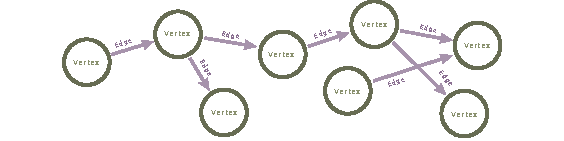
\includegraphics[width=1\textwidth]{images/chapter2/ExampleGraphnew.pdf}%
	\caption[Example of a graph]{Example of a graph}%
	\label{fig:ExampleGraphnew}%
\end{figure}%

The usual way to picture a graph is by drawing a dot for each vertex and joining two of these dots by a line if the corresponding two vertices form an edge.
It is considered to be irrelevant how the dots and lines are drawn;
Which pairs of vertices form an edge and which do not is all that matters.\sfcite{Diestel2000}

\begin{definition}[of adjacent, neighbor vertices]\label{definition:ofadjacentneighborvertices}
	A graph is a pair $ G = \left(V, E \right) $ of sets satisfying $ E \subseteq \left[ V \right]^2 $.
	Two vertices $ x $, $ y $ of $ G $ are \textit{adjacent}, or \textit{neighbors}, if $ xy $ is an edge of $ G $. Two edges $ e \neq f $ are \textit{adjacent} if they have an end in common. If all the vertices of $ G $ are pairwise adjacent, then $ G $ is \textit{complete}.\sfcite{Diestel2000}
\end{definition}

\begin{definition}[of the order of a graph]\label{definition:oftheorderofagraph}
	The number of vertices of a graph $ G $ is its order, written as $ \vert G \vert $;
	its number of edges is denoted by $ \Vert G \Vert $.
	Graphs are \textit{finite} or \text{infinite} according to their order;\sfcite{Diestel2000}
\end{definition}

The graphs considered in this thesis are all finite.

\subsubsection{Directed graphs (Digraphs) and Undirected graphs} \label{subsubsection:LiteratureReview/ShortreviewofGraphTheoryconcepts/Graphs/DirectedgraphsDigraphsandUndirectedgraphs}
\begin{definition}[of directed edges]\label{definition:ofdirectededges}
	A \textit{directed edge} is an edge $ e $ one of whose endpoints is designated as the \textit{tail}, and whose other \textit{endpoint} is designated as the head. They are denoted $ head\left(e\right) $ and $ tail\left(e\right) $, respectively.
	
	A directed edge is said to be \textit{directed from} its tail and \textit{directed to} its head. In a line drawing, the arrow points toward the head.\sfcite{GrossYellenZhang2014}
\end{definition}

\begin{definition}[of digraphs or directed graphs]\label{definition:ofdigraphsordirectedgraphs}
	A \textit{digraph} (or \textit{directed graph}) $ G = \left(V, E\right) $ is a graph each one of its edges is directed. It consists of a finite, nonempty set of vertices $ V $ and a set of edges $ E $, each edge is an ordered pair $ \left(v, w\right) $ of vertices. \sfcite{GrossYellenZhang2014}
\end{definition}

\begin{figure}[H]%
	\centering%
	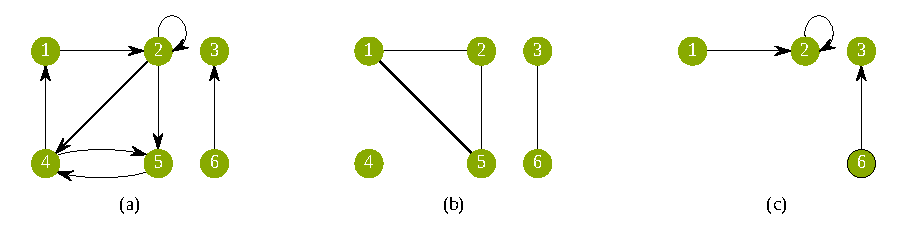
\includegraphics[width=1\textwidth-4pt,%
		bgcolor=white,%
		cfbox=lightestgray % color
			  2pt % rule width
			  0pt % rule separation
			  0pt % margin
	]{images/chapter2/CormenLeisersonRivestStein2009digraphpage1169.pdf}%
	\caption[Directed and undirected graphs]{Directed and undirected graphs. (a) A digraph. (b) An undirected graph. (c) The subgraph of the graph in (a) induced by the set $ \left\{1, 2, 3, 6\right\} $\sfcite{CormenLeisersonRivestStein2009}}%
	\label{fig:CormenLeisersonRivestStein2009digraphpage1169}%
\end{figure}%

\begin{definition}[of undirected graphs]\label{definition:ofundirectedgraphs}
	An \textit{undirected graph} $ G = \left(V, E\right) $ consists of a finite, nonempty set of vertices $ V $ and a set of edges $ E $, each edge is a set $ \left\{v, w\right\} $ of vertices. \sfcite{GrossYellenZhang2014}
\end{definition}

\subsubsection{Walks, paths, trails, cycles and connected graphs} \label{subsubsection:LiteratureReview/ShortreviewofGraphTheoryconcepts/Graphs/WalksPathstrailscyclesandconnectedgraphs}
\begin{definition}[of walks]\label{definition:ofwalks}
	A \textit{walk} of length $ k $ in a graph is a succession of $ k $ edges of the form
	\begin{equation} \stepcounter{equation} \label{equation:ofwalks}
        x_0x_1,\ x_1x_3,\ x_3x_7,\ \ldots, x_{k-1}x_k .
        \tag{\thechapter.\arabic{equation}} % Use \tag{\thechapter.\arabic{equation}} for chapternumber.equationnumber or \tag{\thesection.\arabic{equation}} for chapternumber.sectionnumber.equationnumber or \tag{\thesubsection.\arabic{equation}} for chapternumber.sectionnumber.subsectionnumber.equationnumber
    \end{equation}
    
	and is referred to as a walk between $ x_0 $ and $ x_k $. \sfcite{AldousWilson2000}
\end{definition}

\begin{figure}[H]%
	\centering%
	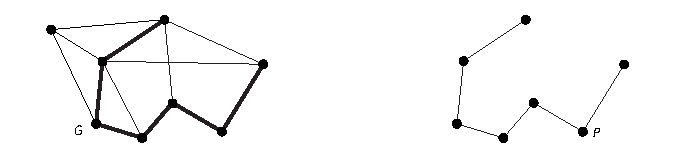
\includegraphics[width=1\textwidth-4pt,%
		bgcolor=white,%
		cfbox=lightestgray % color
			  2pt % rule width
			  0pt % rule separation
			  0pt % margin
	]{images/chapter2/Diestel2000PathPage6.pdf}%
	\caption[A path $ P = P^6 $ in $ G $]{A path $ P = P^6 $ in $ G $\sfcite{Diestel2000}}%
	\label{fig:Diestel2000PathPage6}%
\end{figure}%

\begin{definition}[of walks, \textnormal{another one}]\label{definition:ofwalks2}
	Another definition is in the form of a non-empty alternating sequence
	\begin{equation} \stepcounter{equation} \label{equation:ofwalks2}
        x_0e_0x_1e_1\ldots e_{k-1}x_k
        \tag{\thechapter.\arabic{equation}} % Use \tag{\thechapter.\arabic{equation}} for chapternumber.equationnumber or \tag{\thesection.\arabic{equation}} for chapternumber.sectionnumber.equationnumber or \tag{\thesubsection.\arabic{equation}} for chapternumber.sectionnumber.subsectionnumber.equationnumber
    \end{equation}
    
	of vertices and edges in $ G $ such that $ e_i = \left\{ v_i,\ v_{i+1} \right\} $ for all $ i < k $.
	If $ v_0 = v_k $ the walk is \textit{closed}. \sfcite{Diestel2000}
\end{definition}

\begin{definition}[of trails]\label{definition:oftrails}
	A \textit{trail} is a walk in which all the edges, but not necessarily all the vertices, are different. \sfcite{AldousWilson2000}
\end{definition}

\begin{definition}[of paths]\label{definition:ofpaths}
	A \textit{path} is a non-empty graph $ P = \left( V, E \right) $ of the form
	\begin{equation} \stepcounter{equation} \label{equation:ofpaths}
        V = \left\{ x_0,\ x_1,\ \ldots,\ x_k \right\}, \quad E = \left\{ x_0x_1,\ x_1x_2,\ \ldots,\ x_{k-1}x_{k} \right\}
        \tag{\thechapter.\arabic{equation}} % Use \tag{\thechapter.\arabic{equation}} for chapternumber.equationnumber or \tag{\thesection.\arabic{equation}} for chapternumber.sectionnumber.equationnumber or \tag{\thesubsection.\arabic{equation}} for chapternumber.sectionnumber.subsectionnumber.equationnumber
    \end{equation}
    
	where the vertices $ x_i $ and the edges $ x_{i}x_{i+1} $ are all distinct.
	The vertices $ x_0 $ and $ x_k $ are \textit{linked} by $ P $ and are called its \textit{ends};
	the vertices $ x_1,\ \ldots,\ x_{k-1} $ are the \textit{inner} vertices of $ P $.
	The number of edges of a path is its \textit{length} and the path of length $ k $ is denoted by $ P^k $.
	As $ k $ is allowed to be zero, $ P^0 = K^1 $. \sfcite{Diestel2000}
\end{definition}

\begin{definition}[of cycles]\label{definition:ofcycles}
	As with paths, a cycle is often denoted by its (cyclic) sequence of vertices;
	A cycle C might be written as $ x_0x_1$ $ \ldots $ $ x_{k-1}x_0 $.
	The length of a cycle is its number of edges (or vertices);
	A cycle of length $ k $ is called a \textit{k-cycle} and denoted by $ C^k $.
	
	The minimum length of a cycle in a graph $ G $ is the \textit{girth} $ g\left(G\right) $ of $ G $;
	the maximum length of a cycle in $ G $ is its \textit{circumference}.
	If G does not contain a cycle, the former is set to $ \infty $, the latter to zero.
	An edge that joins two vertices of a cycle but is not itself an edge of the cycle is a \textit{chord} of that cycle.\sfcite{Diestel2000}
\end{definition}

\begin{theorem}[on edge set partitioning into cycles] \label{theorem:onedgesetpartitioningintocycles}
	The edge set of a graph can be partitioned into \glspl{cycle} if, and only if, every vertex has even degree.\sfcite{Bollobas1998}
\end{theorem}

\begin{proof}[of \autoref{theorem:onedgesetpartitioningintocycles}] \label{proof:onedgesetpartitioningintocycles}
	See \citetitle{Bollobas1998} - \citeauthor{Bollobas1998} (\citeyear{Bollobas1998}), page 5.
\end{proof}

\begin{definition}[of connected graphs]\label{definition:ofconnectedgraphs}
	A graph is \textit{connected} if there is a path between each pair of vertices, and is \textit{disconnected} otherwise.
	
	An edge in a connected graph is a \textit{bridge} if its removal leaves a disconnected graph. Every disconnected graph can be split up into a number of connected subgraphs, called \textit{components}. \sfcite{AldousWilson2000}
\end{definition}

\begin{theorem}[on the presence of triangles in a graph] \label{theorem:onthepresenceoftrianglesinagraph}
	Every graph of order $ n $ and size greater than $ \lfloor frac{n^2}{4} \rfloor $ contains a triangle.\sfcite{Bollobas1998}
\end{theorem}

\begin{proof}[of \autoref{theorem:onthepresenceoftrianglesinagraph}] \label{proof:onthepresenceoftrianglesinagraph}
	See \citetitle{Bollobas1998} - \citeauthor{Bollobas1998} (\citeyear{Bollobas1998}), page 6.
\end{proof}

\begin{corollary}[on spanning trees of connected graphs] \label{theorem:onspanningtreesofconnectedgraphs}
	Every connected graph contains a spanning tree.\sfcite{Bollobas1998}
\end{corollary}

\begin{figure}[H]%
	\centering%
	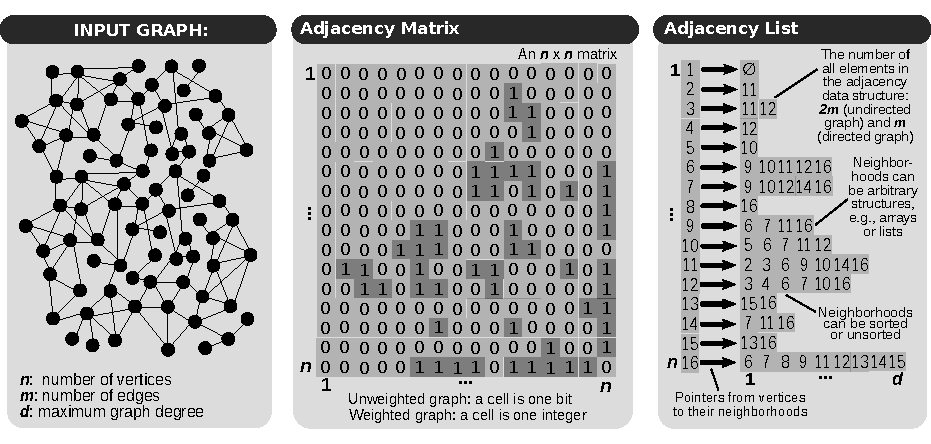
\includegraphics[width=1\textwidth,%
	]{images/chapter2/BestaPeterGerstenbergerFischerPodstawskiBarthelsAlonsoHoefler2019adjacencylistpage8.pdf}%
	\caption[Illustration of Adjacency Matrix and Adjacency List]{Illustration of Adjacency Matrix and Adjacency List\sfcite{BestaPeterGerstenbergerFischerPodstawskiBarthelsAlonsoHoefler2019}}%
	\label{fig:BestaPeterGerstenbergerFischerPodstawskiBarthelsAlonsoHoefler2019adjacencylistpage8}%
\end{figure}%

\paragraph{Adjacency lists and adjacency matrix}\mbox{}\\\indent
	There exist two standard ways to represent a graph: as a collection of \textit{adjacency lists} or as an \textit{adjacency matrix};
	both valid for either directed and undirected graphs.
	The adjacency-list representation provides a compact way to represent \textit{sparse} graphs, that is those for which $ \vert E \vert $ is much less than $ \vert V \vert ^2 $;
	when instead a graph is \textit{dense} (i.e. $ \vert E \vert $ is close to $ \vert V \vert ^2 $), the adjacency matrix could be used for optimization purposes.
	The adjacency-matrix representation of a graph $ G = \left( V, E \right) $ assumes that vertices are numbered $1, 2, \ldots, \vert V \vert $ in some arbitrary manner - consists of a $ \vert V \vert \times \vert V \vert $ matrix $ A = \left( a_{ij} \right) $ such that $ a_{ij} = 1 $ if $ \left(i, j \right) \in E $; $ 0 $ otherwise. \sfcite{CormenLeisersonRivestStein2009}
		
	An example is shown in \hyperref[fig:BestaPeterGerstenbergerFischerPodstawskiBarthelsAlonsoHoefler2019adjacencylistpage8]{\autoref{fig:BestaPeterGerstenbergerFischerPodstawskiBarthelsAlonsoHoefler2019adjacencylistpage8}}.
\par
\subsubsection{Notes on terminology used}\label{subsubsection:Notesonterminology}
\begin{remark}[on nodes]\label{remark:onnodes}
		Nodes and vertices are used interchangeably and represent the constituting discrete elements of a graph.
\end{remark}
	
\begin{remark}[on edges]\label{remark:onedges}
	Edges, hops, links and arcs are used interchangeably and represent relationships and connections among vertices.
\end{remark}
	
\begin{remark}[on depth and number of hops]\label{remark:ondepthandnumberofhops}
	Depth, level and distance are used interchangeably and represent the number of hops from a vertex to another given reference vertex.
\end{remark}
	
\begin{remark}[on connected nodes]\label{remark:onconnectednodes}
	If a single edge connects two nodes, they are considered to be directly connected.
	If the pathways connecting two nodes have more than one edge, they are indirectly connected;
	that is, there is at least another vertex on the road between them.
\end{remark}
	
\begin{remark}[on paths]\label{remark:onpaths}
	A route is a path that begins at one source node and leads to a destination node by traversing consecutive edges (either in the same direction or not).
\end{remark}
	
\begin{remark}[on outbound and inbound directions]\label{remark:onoutboundandinbounddirections}
	If an edge's direction points away from the node being analyzed, it is said to have outbound or outgoing direction.
	If an edge's direction points exactly to the reference node, it has inbound or incoming direction.
\end{remark}
	
\begin{remark}[on directed paths]\label{remark:ondirectedpaths}
	A path made up of just edges with the same concordant direction will be called a directed path; an undirected path, on the other hand, is a path made up of edges with no constraints on their relative directions.
	An outgoing path, for example, begins at the beginning node and consists solely of outgoing edges with respect to the path's vertices;
	an ingoing path, on the other hand, consists solely of ingoing edges.
\end{remark}
	
\begin{remark}[on descendants]\label{remark:ondescendants}
	The nodes that can be reached by the original node via outgoing paths will be referred to as descendants.
	This set includes an initial node's children, as well as their children, and so on.
\end{remark}
	
\begin{remark}[on neighbors]\label{remark:onneighbors}
	Those nodes that are directly related to the reference node, regardless of the direction of the edges involved, will be named neighbors.
\end{remark}
	
\begin{remark}[on cycles]\label{remark:oncycles}
	A directed path that starts and finishes with the same node is called a cycle.
	Therefore, if a path has the same vertex more than once it is said to contain a cycle.
	It is worth noting that the definition is based on avoiding multiple visits of the same vertex rather than multiple walks on the same arc. 
	Furthermore, an undirected path that passes across the same node more than once does not mean it contains a cycle, because it is only an aggregation of different directed paths (though one of them could be a cycle;
	in such case, the path effectively contains a cycle).
\end{remark}
	
\begin{remark}[on fathers and children]\label{remark:onfathersandchildren}
	Will be called children the nodes that are directly connected to the given node and that can be reached by means of an outbound edge.
	In a dual way, will be called fathers the nodes that are directly connected to the given node and that can be reached by means of an inbound edge.
\end{remark}
	
\begin{remark}[on ancestors and descendants]\label{remark:onancestorsanddescendants}
	The nodes that are reachable from the beginning node via ingoing paths will be referred to as ancestors.
	The set of vertices that can be reached by the given node via outgoing paths can also be defined as ancestors.
	The same is true for descendants.
\end{remark}
	
\begin{remark}[on exploration and traversals]\label{remark:onexplorationandtraversals}
	Graph exploration and traversal are used interchangeably.
\end{remark}

In the next subsection are presented a few examples of usage of graphs to represent real-life interconnected entities.

\subsection{Graph examples} \label{subsection:LiteratureReview/ShortreviewofGraphTheoryconcepts/Graphexamples}
The graph examples taken into consideration in this subsection are:
\setlist{nolistsep} \begin{itemize}[noitemsep]
	\item \gls{road network}s,
	\item \gls{computer network}s,
	\item and \gls{social network}s.
\end{itemize}



\subsubsection[Road networks]{\Glspl{road network}} \label{subsubsection:LiteratureReview/ShortreviewofGraphTheoryconcepts/Graphexamples/Roadnetworks}
A great example of a graph is a road network as shown in \hyperref[fig:WikipediaMilanoMetro2021Graphedit]{\autoref{fig:WikipediaMilanoMetro2021Graphedit}}.\sfcite{WikipediaMilanoMetro2021}.

\begin{figure}[H]%
	\centering%
	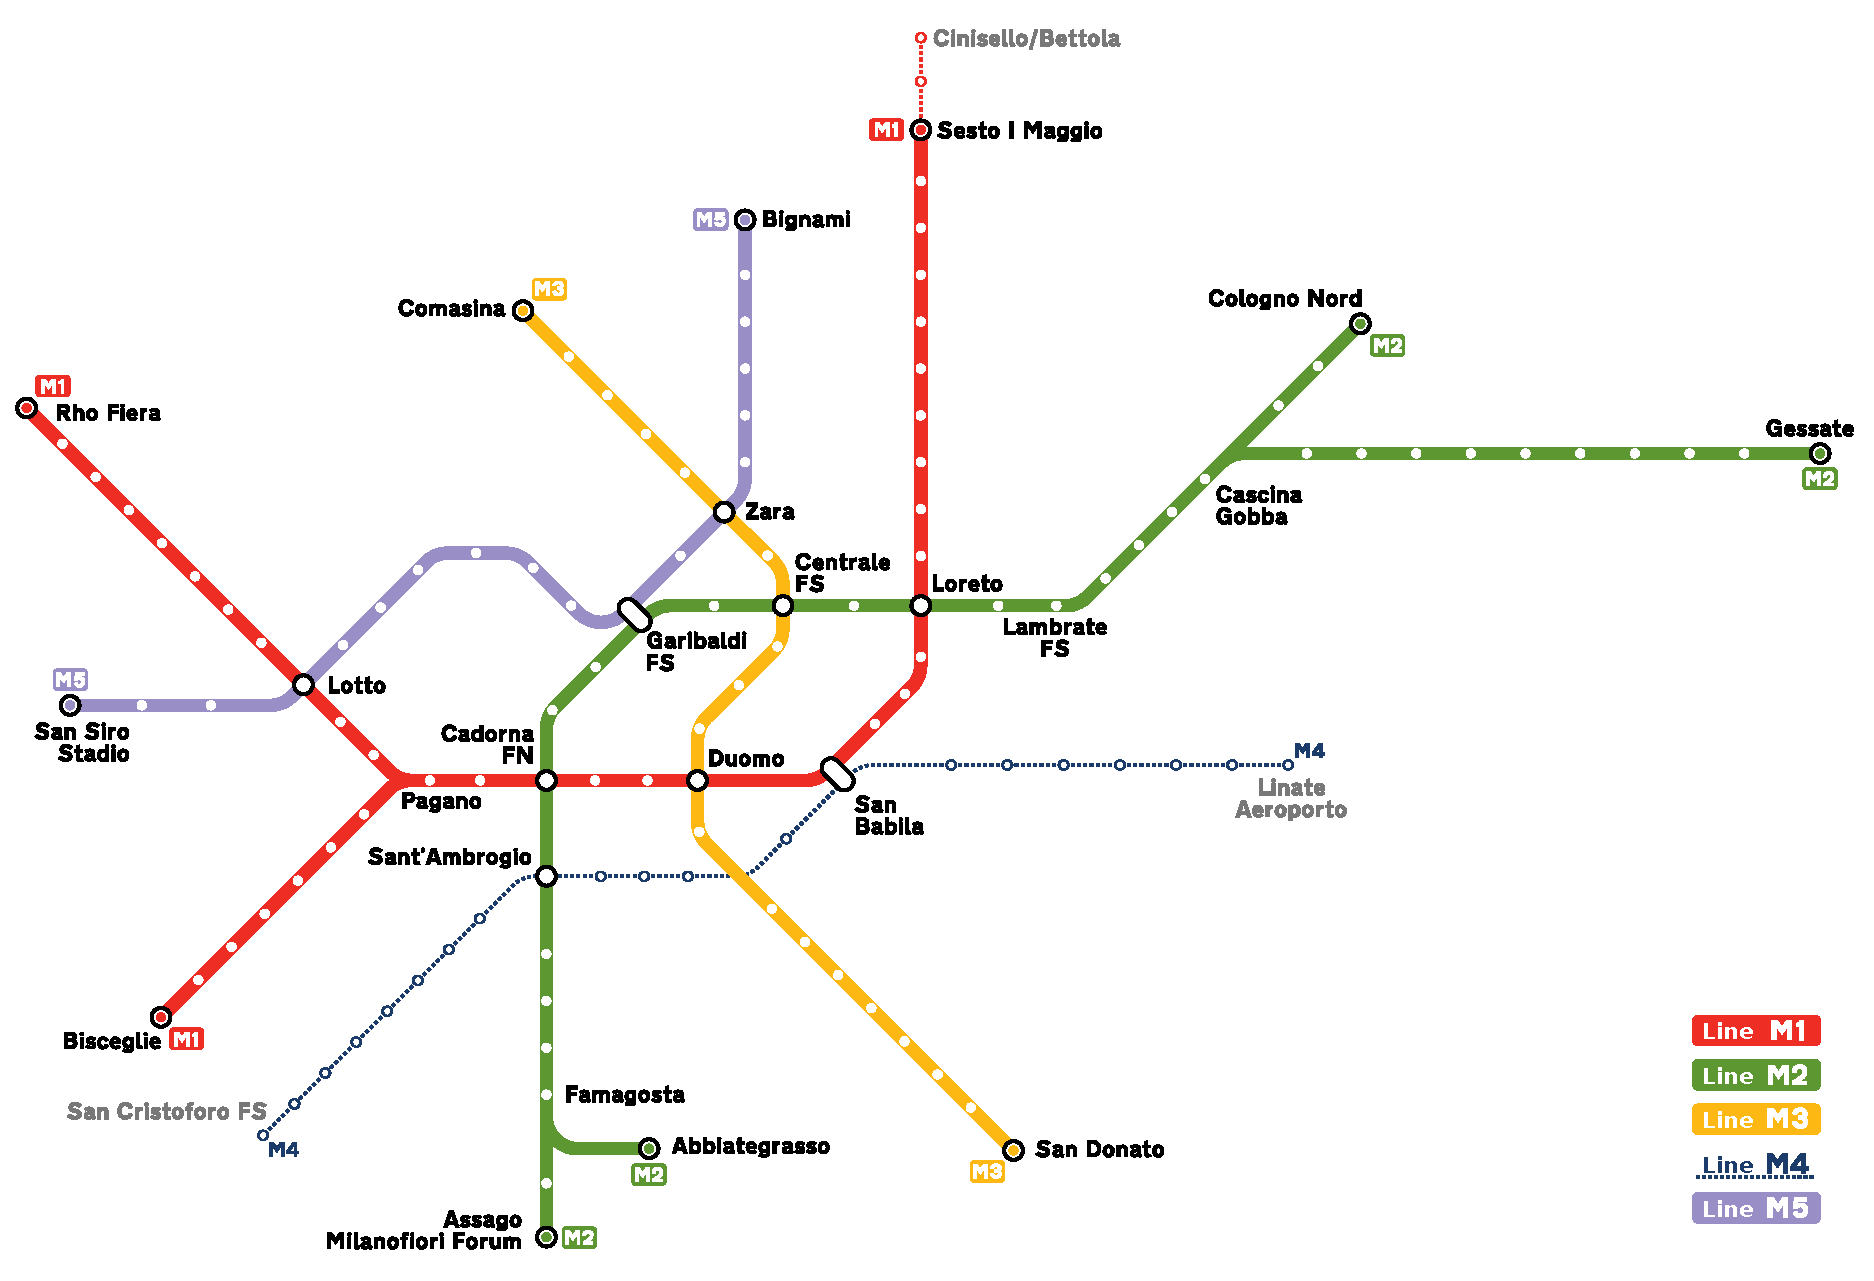
\includegraphics[width=1\textwidth-4pt,%
		bgcolor=white,%
		cfbox=lightestgray % color
			  2pt % rule width
			  0pt % rule separation
			  0pt % margin
	]{images/chapter2/WikipediaMilanoMetro2021Graphedit.pdf}%
	\caption[Network map of Milan Metro stations and lines]{Network map of \gls{Milan} Metro stations and lines\sfcite{WikipediaMilanoMetro2021}}%
	\label{fig:WikipediaMilanoMetro2021Graphedit}%
\end{figure}%

The nodes in such networks are road intersections or stations, stops, while the edges are the actual roadways, railways, airways or seaways.
Graph analysis can address a variety of problems about road networks, including:
\setlist{nolistsep} \begin{enumerate}[noitemsep]
	\item finding various alternative routes?
	\item the shortest path's length;
	\item a way to visit all the vertices in a list in the shortest time possible;
	\item the shortest path from one location to another.
\end{enumerate}
The third topic is particularly significant for \gls{postal delivery}, as it helps reduce the distance traveled while increasing the number of shipments delivered.\sfcite{Scifo2020}

\subsubsection{Computer networks} \label{subsubsection:LiteratureReview/ShortreviewofGraphTheoryconcepts/Graphexamples/Computernetworks}
In computer networks, computers and routers can be considered as vertices and cables, routing lines connecting them are indeed the links (of a graph).
The following are some of the common questions that emerge with this type of network structure:
\setlist{nolistsep} \begin{itemize}[noitemsep]
	\item A shortest path problem:
	how quickly can data be transferred from point A to point B?
	\item Node centrality algorithms: which of the vertices is the most important or critical one?
\end{itemize}
For more details on the algorithms, see \hyperref[subsection:LiteratureReview/ShortreviewofGraphTheoryconcepts/Graphanalysisandalgorithms]{\S\ \ref{subsection:LiteratureReview/ShortreviewofGraphTheoryconcepts/Graphanalysisandalgorithms} - \nameref{subsection:LiteratureReview/ShortreviewofGraphTheoryconcepts/Graphanalysisandalgorithms}} on \hyperref[subsection:LiteratureReview/ShortreviewofGraphTheoryconcepts/Graphanalysisandalgorithms]{page \pageref{subsection:LiteratureReview/ShortreviewofGraphTheoryconcepts/Graphanalysisandalgorithms}}. \sfcite{Scifo2020}

\subsubsection{Social networks} \label{subsubsection:LiteratureReview/ShortreviewofGraphTheoryconcepts/Graphexamples/Socialnetworks}
Graphs are used by \gls{Facebook}, \gls{LinkedIn}, and many other social media platforms to model their users and interactions.
Nodes represent persons and edges show their \textit{friendship} or \textit{professional} relationship in the most basic example of a social graph, as shown in figure \hyperref[fig:SocialNetwork]{\autoref{fig:SocialNetwork}}.

\begin{figure}[H]%
	\centering%
	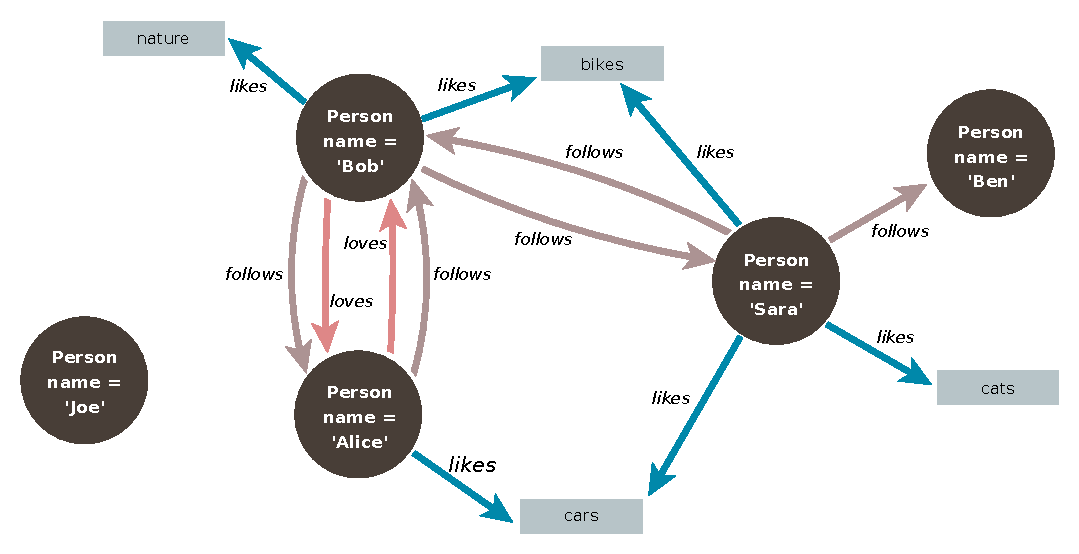
\includegraphics[width=1\textwidth]{images/chapter2/SocialNetwork.pdf}%
	\caption[Example of a social network graph]{Example of a social network graph}%
	\label{fig:SocialNetwork}%
\end{figure}%

For instance, when looking at someone's profile on \gls{LinkedIn}, it is possible to see the degree of connection of that profile from the logged-in user.
If \textit{3rd} is shown on that profile, it means that the logged-in user is just two connections away from the viewed profile.
In other words, one person in the logged-in user's network is already connected to a person who is connected to the viewed profile.\sfcite{Scifo2020}

\subsection{Graph analysis and algorithms} \label{subsection:LiteratureReview/ShortreviewofGraphTheoryconcepts/Graphanalysisandalgorithms}
In this section are presented some methods of analysis that are at the very core of graph algorithms.

\subsubsection[Centrality (Node importance)]{\gls{Centrality} (\gls{Node importance})} \label{subsubsection:LiteratureReview/ShortreviewofGraphTheoryconcepts/Graphanalysisandalgorithms/CentralityNodeimportance}
\gls{Centrality} focuses on understanding which nodes in a network are more important than others.
What exactly does 'importance' mean?
Different forms of centrality algorithms have been developed to evaluate diverse things,\sfcite{NeedhamHodler2021} such as the ability to quickly spread information versus the ability to distinguish critical nodes in computer networks.
By critical, it is meant that if a specific node is not working for some reason, the whole network will be impacted.
Not every node affects the network in the same way.
It comes naturally that backbone nodes are crucially important.

\begin{center}
	\vspace*{-0.25cm}
	\begin{longtable}{p{0.22\linewidth}p{0.3475\linewidth}p{0.3475\linewidth}}
		\hline \hline
		\textbf{Algorithm type} & \textbf{What it does} & \textbf{Usecases}\\
		\hline \hline
		\endfirsthead
		
		\multicolumn{3}{l}{... continued from previous page}\\
		\hline \hline
		\textbf{Algorithm type} & \textbf{What it does} & \textbf{Usecases}\\
		\hline \hline
		\endhead
		
		\hline
		\caption*{\tablename\ \thetable{}: \nameref*{longtable:centralityalgorithms}\sfcite{NeedhamHodler2021}. Continues on next page ...}
		\vspace*{0.5cm}
		\endfoot
		
		\hline
		%\multicolumn{2}{| c |}{End of Table}\\
		%\hline
		\caption[Overview of centrality algorithms]{Overview of centrality algorithms\sfcite{NeedhamHodler2021}}\label{longtable:centralityalgorithms}
		\vspace*{0.5cm}
		\endlastfoot

		\textbf{Degree Centrality} & Calculates how many edges a vertex is connected to & Quantification of a person's popularity\\
		\hline
		\textbf{Closeness Centrality, Was\-ser\-man and Faust, Har\-mo\-nic Cen\-tra\-li\-ty} & Determines which vertices have the shortest paths to all other vertices & Choosing optimal location of new public facilities for maximum accessibility\\
		\hline
		\textbf{Betweenness Cen\-tra\-li\-ty, Ran\-do\-mi\-zed-Ap\-pro\-xi\-ma\-te Brandes} & Calculates how many shortest paths pass through a vertex & Finding the control genes for specific diseases for better drug targeting\\
		\hline
		\textbf{All Pairs Shortest Path} & Computes the shortest path between all pairs of nodes in the graph & Finding alternate routes around traffic jams\\
		\hline
		\textbf{PageRank} & Quantifies a vertex's importance from its connections with the neighbors and their neighbors (popularized by \gls{Google}) & Rating text for entity relevance in natural language processing and identifying the most relevant features for extraction in machine learning.\\
		\hline
	\end{longtable}
	\vspace*{-1.35cm}
\end{center}

In the case of social media networks, while it may be possible a cascade reaction, generally it is very unlikely that a single person's retirement from social media makes that whole social community retire.\sfcite{Scifo2020}

\subsubsection[Pathfinding]{\gls{Pathfinding}} \label{subsubsection:LiteratureReview/ShortreviewofGraphTheoryconcepts/Graphanalysisandalgorithms/Pathfinding}
For graph analytics and algorithms, paths are fundamental.
Finding the \gls{shortest path}s is perhaps the most common task performed with graph algorithms and it is a prerequisite for a variety of analyses.
The shortest path is an exploration route with the least hops or lowest weight.
If the graph is directed, the shortest path between two nodes is determined by the direction of the relationships.\sfcite{NeedhamHodler2021}

An example is shown in \hyperref[fig:GrowingwiththeWebImms2021Pathfinding]{\autoref{fig:GrowingwiththeWebImms2021Pathfinding}}.\sfcite{GrowingwiththeWebImms2021}

\begin{figure}[H]%
	\centering%
	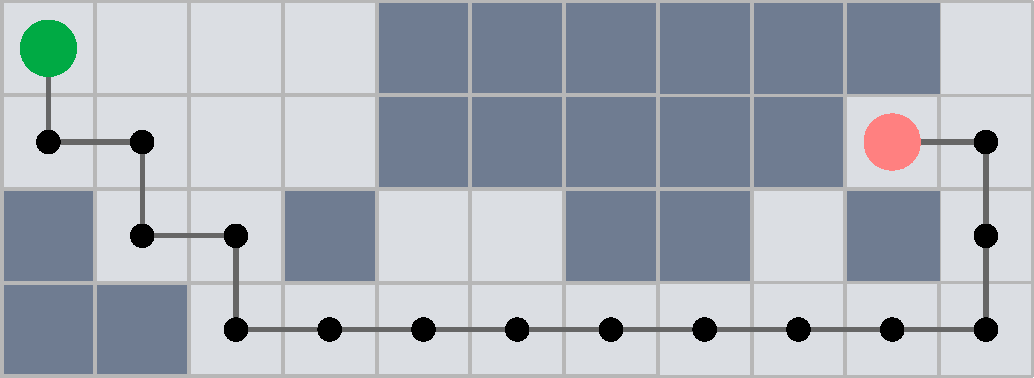
\includegraphics[width=1\textwidth]{images/chapter2/GrowingwiththeWebImms2021Pathfinding.pdf}%
	\caption[An illustration of the directional movements during the execution of a shortest path algorithm, in a maze]{An illustration of the directional movements during the execution of a shortest path algorithm, in a maze\sfcite{GrowingwiththeWebImms2021}}%
	\label{fig:GrowingwiththeWebImms2021Pathfinding}%
\end{figure}%

\paragraph{Path types}\mbox{}\\\indent
The \textit{average shortest path} is used to evaluate a network's overall efficiency and resiliency, for example in determining the average distance between subway stations.
Sometimes it may be necessary to get the longest optimized route for cases where is requested to know which subway stations are farthest apart or have the most number of stops between them, even when the best route is chosen.
The \textit{diameter} would be used in this case to discover the longest shortest path between all node pairs.\sfcite{NeedhamHodler2021}

\begin{center}
	\vspace*{-0.25cm}
	\begin{longtable}{p{0.22\linewidth}p{0.3475\linewidth}p{0.3475\linewidth}}
		\hline \hline
		\textbf{Algorithm type} & \textbf{What it does} & \textbf{Usecases}\\
		\hline \hline
		\endfirsthead
		
		\multicolumn{3}{l}{... continued from previous page}\\
		\hline \hline
		\textbf{Algorithm type} & \textbf{What it does} & \textbf{Usecases}\\
		\hline \hline
		\endhead
		
		\hline
		\caption*{\tablename\ \thetable{}: \nameref*{longtable:pathfindingandgraphsearchalgorithms}\sfcite{NeedhamHodler2021}. Continues on next page ...}
		\vspace*{0.5cm}
		\endfoot
		
		\hline
		%\multicolumn{2}{| c |}{End of Table}\\
		%\hline
		\caption[Overview of pathfinding and graph search algorithms]{Overview of pathfinding and graph search algorithms\sfcite{NeedhamHodler2021}}\label{longtable:pathfindingandgraphsearchalgorithms}
		\vspace*{0.5cm}
		\endlastfoot

		\textbf{Breadth First Search}\sfcite{WikipediaBreadthfirstsearch2021} & Tree traversal by exploring right the nearest neighbors first and then the sublevel neighbors & GPS systems locating neighbor vertices to identify nearby places of interest\\
		\hline
		\textbf{Depth First Search}\sfcite{WikipediaDepthfirstsearch2021} & Tree traversal by exploring down the sublevel neighbors first before backtracking & Optimal solution path discovery with hierarchical choices\\
		\hline
		\textbf{Shortest Path} & Computes the shortest path between two vertices & Driving route discovery between two locations\\
		\hline
		\textbf{All Pairs Shortest Path} & Computes the shortest path between every two vertices of the graph & Finding alternate routes around a traffic jam\\
		\hline
		\textbf{Single Source Shor\-t\-est Path} & Computes the shortest path between a root vertex and all other vertices & Least cost routing of phone calls\\
		\hline
		\textbf{Minimum Spanning Tree} & Computes the path in a connected tree structure that has the smallest cost for visiting all vertices & Routing optimization or garbage collection\\
		\hline
		\textbf{\gls{Random Walk}} & Returns a list of vertices along a path of specified size by randomly choosing relationships to traverse. & Augmenting training for machine learning.\\
		\hline
	\end{longtable}
	\vspace*{-1.35cm}
\end{center}
\par

\subsubsection{Community detection} \label{subsubsection:LiteratureReview/ShortreviewofGraphTheoryconcepts/Graphanalysisandalgorithms/Communitydetection}
Community detection, often referred to as clustering, is a method of finding a group of nodes sharing certain characteristics.
\sfcite{Scifo2020}

Usually, real-world networks present substructures (often quasi-fractal) of almost independent subgraphs.
Connectivity is utilized to detect communities and quantify the quality of clustering groupings.
Analyzing different types of communities within a graph can uncover structures, like hubs, hierarchies and tendencies of groups to attract or repel others.
These techniques are also used to study emergent phenomena such as echo chambers and filter bubble effects.\sfcite{NeedhamHodler2021}

This topic is thoroughly presented in \hyperref[chapter:CommunityDetection]{\S\ \ref{chapter:CommunityDetection} - \nameref{chapter:CommunityDetection}} on \hyperref[chapter:CommunityDetection]{page \pageref{chapter:CommunityDetection}} where also the execution of the Label Propagation Community Detection algorithm is step-by-step explained.

\subsubsection{Link prediction} \label{subsubsection:LiteratureReview/ShortreviewofGraphTheoryconcepts/Graphanalysisandalgorithms/Linkprediction}
Using intelligent models, it is possible to predict whether two vertices of a graph shall be connected in the future or not.

Once again, perfect examples of applications of link prediction are recommendation engines.\sfcite{Scifo2020}

\subsubsection{Other algorithms and problems in Graph Theory} \label{subsection:LiteratureReview/ShortreviewofGraphTheoryconcepts/Graphanalysisandalgorithms/OtheralgorithmsandproblemsinGraphTheory}
While the problems and algorithms treated above are just a taste of only the most commonly known and often considered problems in graph theory literature, there is however a vast majority of other problems that are not presented here.
The focus of this thesis is limited to a precise problem.
Thus, for more on these topics, refer to graph theory books and scientific literature.

\section{Review of Graph Database Systems} \label{section:LiteratureReview/ReviewofGraphDatabaseSystems}
Graph databases address one of today's most important macroeconomic trends:
generating insight and competitive advantage by harnessing complex and dynamic relationships in highly connected data.
Whether it is understanding network elements, customer relationships, genes  and proteins, or entertainment producers and consumers, the ability to understand and analyze vast graphs of highly connected data will be critical in determining which companies outperform their competitors over the next decade.

Graph databases are the most effective way to represent and query connected data.
In order to interpret and understand connected data's value, first is needed to understand how its constituent elements are interconnected.
Most of the time, naming and qualifying the relationships between things is needed to produce this understanding.

Despite the fact that huge corporations got this a long time ago and began developing their own proprietary graph processing technologies, today, technology has rapidly become democratized.
General-purpose graph databases are now available, allowing ordinary people to profit from connected data without having to invest in their own graph infrastructure.\sfcite{RobinsonWebberEifrem2015}

Graphs have long been recognized as a natural manner of representing information and knowledge and the concept of a "graph database" has been around since at least the 1980s.
However, because of the technological advancements, it is only lately possible to take full advantage of this abstract concept.\sfcite{AnglesGutierrez2018}
	
Graph databases have since been used to tackle major challenges in social networking, recommendation systems, geospatial/GIS, master data management and many other domains.
The massive commercial success of companies like \gls{Facebook}, \gls{Google}, and \gls{Twitter}, all of which have built their business models around their own proprietary graph technologies, and the introduction of general-purpose graph databases into the technology landscape, are driving this increased focus on graph databases.
This is clearly visible in the popularity change chart of different database systems categories shown in \hyperref[fig:solid2021popularitychange]{\autoref{fig:solid2021popularitychange}}.\sfcite{solid2021}

\begin{figure}[H]%
	\centering%
	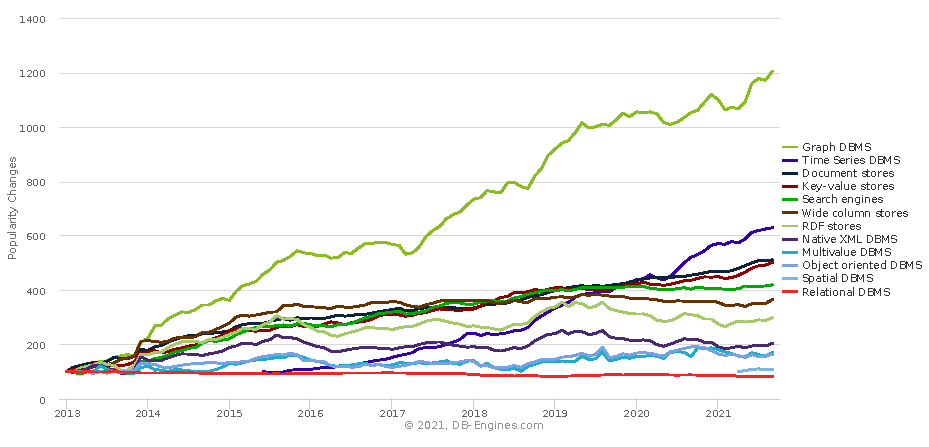
\includegraphics[width=1\textwidth-4pt,%
		bgcolor=white,%
		cfbox=lightestgray % color
			  2pt % rule width
			  0pt % rule separation
			  0pt % margin
	]{images/chapter2/solid2021popularitychange.pdf}%
	\caption[Trend of DBMS popularity changes per category]{Trend of DBMS popularity changes per category\sfcite{solid2021}}%
	\label{fig:solid2021popularitychange}%
\end{figure}%

It is interesting to see what makes graph databases so compelling.
To that end in the following subsection are presented some general notions, definitions of graph databases.
Follows in \hyperref[subsection:LiteratureReview/ReviewofGraphDatabaseSystems/Graphdatamodels]{\S\ \ref{subsection:LiteratureReview/ReviewofGraphDatabaseSystems/Graphdatamodels} - \nameref{subsection:LiteratureReview/ReviewofGraphDatabaseSystems/Graphdatamodels}} a panoramic description of graph data models.
After that in \hyperref[subsection:LiteratureReview/ReviewofGraphDatabaseSystems/Graphdatabasecharacteristics]{\S\ \ref{subsection:LiteratureReview/ReviewofGraphDatabaseSystems/Graphdatabasecharacteristics} - \nameref{subsection:LiteratureReview/ReviewofGraphDatabaseSystems/Graphdatabasecharacteristics}} the main characteristics of graph databases are investigated and in \hyperref[subsection:LiteratureReview/ReviewofGraphDatabaseSystems/GraphQueryLanguages]{\S\ \ref{subsection:LiteratureReview/ReviewofGraphDatabaseSystems/GraphQueryLanguages} - \nameref{subsection:LiteratureReview/ReviewofGraphDatabaseSystems/GraphQueryLanguages}} an overview of the various graph query languages is presented.
During the work of this thesis isn't done any benchmarking activity \textit{per sé}.
But to better understand the differences between graph databases, some comparisons, benchmarks are be presented between GDBMSs in \hyperref[subsection:LiteratureReview/ReviewofGraphDatabaseSystems/GDBMSscomparison]{\S\ \ref{subsection:LiteratureReview/ReviewofGraphDatabaseSystems/GDBMSscomparison} - \nameref{subsection:LiteratureReview/ReviewofGraphDatabaseSystems/GDBMSscomparison}}.
That shall be the closing of this chapter.

\subsection{Different definitions of graph databases} \label{subsection:LiteratureReview/ReviewofGraphDatabaseSystems/Differentdefinitionsofgraphdatabases}
There does not seem to be a universally accepted definition of what constitutes a graph database.

A common definition is the following:
\begin{definition}[of graph databases, \textnormal{common}]\label{definition:ofgraphdatabasescommon}
	A graph database is a database that organizes data by modeling it by means of the concepts of vertices and edges, where vertices represent the entities to be stored and edges represent the relationships that exist among nodes.\sfcite{Sinico2017}
\end{definition}

A more specific definition is:

\begin{definition}[of graph databases, \textnormal{specific}]\label{definition:ofgraphdatabasesspecific}
	A graph database is any storage system that has the following properties:
	\setlist{nolistsep} \begin{itemize}[noitemsep]
		\item is designed to store graph-like data;
		\item organizes data by means of node and edge elements;
		\item provides built-in graph traversal functions;
		\item (hopefully) provides graph data integrity;
	\end{itemize}
\end{definition}

which is very similar to the definition provided in \citetitle{AnglesGutierrez2018} by \citeauthor{AnglesGutierrez2018} (\citeyear{AnglesGutierrez2018}):

\begin{definition}[of graph databases, \textnormal{by Angles and Gutierrez}]\label{definition:ofgraphdatabasesbyAnglesandGutierrez}
	A graph database is a database where the data structures for the schema and/or instances are modeled as a graph, where \gls{data manipulation} is expressed by graph-oriented operations and appropriate integrity constraints can be defined over the graph structure.\sfcite{AnglesGutierrez2018}
\end{definition}

Another definition focused on database requirements is the one that follows:


\begin{definition}[of graph databases, \textnormal{with requirements}]\label{definition:ofgraphdatabaseswithrequirements}
	A graph database is a system with Create, Read, Update, and Delete (CRUD) methods that exposes a graph data model.
	Graph databases are generally built for use with transactional (OLTP) systems.
	Accordingly, they are normally optimized for transactional performance and engineered with transactional integrity and operational availability
	in mind.\sfcite{RobinsonWebberEifrem2015}
\end{definition}

One last definition shall be reported and that revolves around the idea a graph database has to provide index-free adjacency:

\begin{definition}[of graph databases, \textnormal{requiring index-free adjacency}]\label{definition:ofgraphdatabasesrequiringindexfreeadjacency}
	A graph database is a database that uses graph structures with vertices, edges and properties to represent and store data providing index-free adjacency.\sfcite{IBMSystemG2018, Rodriguez2010}
\end{definition}

On data retrieval, some new concepts and generally a new query language are required, if compared to the standard query language of relational databases.
There is not, yet, a standard query language for this domain:
each graph database product comes with its own query language and, up to now, none of these query languages has risen to prominence in the same fashion as SQL did for relational databases.
Some standardization efforts are however taking place, leading to systems like \textit{Gremlin} (which works with a variety of graph engines that use the property graph model) and \textit{SPARQL} (which is used in RDF graphs). \sfcite{WikipediaGraphDatabase2021}

In a more general sense, a database model (or just data model) is a conceptual tool used to model representations of real world entities and the relationships among them. 
As is well known, a data model can be characterized by three basic components, namely:
\setlist{nolistsep} \begin{enumerate}[noitemsep]
	\item data structures;
	\item query and transformation language;
	\item integrity constraints.
\end{enumerate}

Following this definition:

\begin{definition}[continues={definition:ofgraphdatabasesbyAnglesandGutierrez}]\label{definition:ofgraphdatabasesbyAnglesandGutierrezcontinued}
	A graph database model is a model where data structures for the schema and/or instances are modeled as graphs (or generalizations of them), where the \gls{data manipulation} is expressed by graph-oriented operations (i.e. a graph query language) and appropriate integrity constraints can be defined over the graph structure. \sfcite{AnglesGutierrez2018}
\end{definition}

Having given some definitions of what are commonly considered to be graph databases, in the next subsection graph data models shall be described.

\subsection{Graph data models} \label{subsection:LiteratureReview/ReviewofGraphDatabaseSystems/Graphdatamodels}
When it comes to graph databases, there are a variety of features that may be considered.
The data model that they use is one of them.
Property graphs, RDF graphs, and hypergraphs are the three most used graph data models.\sfcite{RobinsonWebberEifrem2015} 
The property graph is more of an industry standard than the RDF model, which is a W3C standard.\sfcite{Seaborne2015}

In the following subsubsections, each of these models is presented in detail.

\subsubsection{Property graph} \label{subsubsection:LiteratureReview/ReviewofGraphDatabaseSystems/Graphdatamodels/Propertygraph}

\begin{definition}[of property graphs]\label{definition:ofpropertygraphs}
	A property graph (see \hyperref[fig:propertygraphneo4j]{\autoref{fig:propertygraphneo4j}}\sfcite{Neo4jGuideDataModeling2021}) is a one that has the following properties:
	\setlist{nolistsep} \begin{itemize}[noitemsep]
		\item It is made up of vertices, edges, attributes and labels - or some similar categorization form.
		\item Vertices can have an arbitrary amount of attributes, typically key-value pairs.
		\item Vertices are connected by edges which structure the graph.
			  Each edge has a direction, a single name, a start vertex and an end vertex.
			  There are no dangling edges.
		\item One or more categories can be applied to vertices and edges, by means of classes or labels.
			  Vertices are grouped together by categories, which describe the functions they perform in the dataset.
			  Edges can be categorized as well.
			  Edge direction and type, category work together to provide semantic meaning to the network structure.
		\item Relationships too can have attributes.
			  The ability to add attributes to them is especially useful for improving the graph's semantics and for limiting the results at query-time.\sfcite{RobinsonWebberEifrem2015}
    \end{itemize}
\end{definition}

\begin{figure}[H]%
	\centering%
	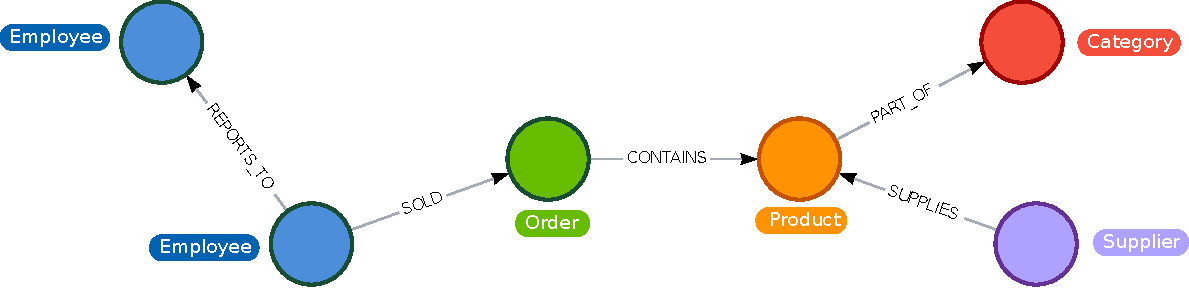
\includegraphics[width=1\textwidth]{images/chapter2/propertygraphneo4j.pdf}%
	\caption[An example of a property graphy]{An example of a property graphy\sfcite{Neo4jGuideDataModeling2021}}%
	\label{fig:propertygraphneo4j}%
\end{figure}%

This type of model has gained a lot of traction and it is used by the majority of the graph DBMSs today.
In addition, the Apache TinkerPop project has sought to create the groundwork for standardization.\sfcite{ApacheTinkerPopWebsite2021, ApacheTinkerPopDocs2021}

\subsubsection{RDF graphs, Ontologies, Inferences, SPARQL, Semantic Web and Linked Data} \label{subsubsection:LiteratureReview/ReviewofGraphDatabaseSystems/Graphdatamodels/RDFgraphsOntologiesInferencesSPARQLSemanticWebandLinkedData}
The formal definition of RDF, given by W3C, is:
\begin{definition}[of RDF]\label{definition:ofRDF}
	Resource Description Framework (RDF) is a standard model for data interchange on the Web.
	RDF has features that make data merging easier even when the underlying schemas are different and it supports schema evolution over time without needing all data consumers to be updated.\sfcite{W3CSemanticWebRDF2014}
\end{definition}

To put it another way, RDF expands the Web's linking structure by allowing URIs to be used to name both relationships between objects and the two ends of the link.
This model is built on a set of triples, each of which consists of a subject, a predicate and an object.
An RDF graph, also known as a triples store, is a collection of such triples.

In an RDF graph, there are three types of vertices:
\setlist{nolistsep} \begin{itemize}[noitemsep]
	\item URI vertices,
	\item literal vertices
	\item and blank vertices.\sfcite{W3CRDFConcepts2014}
\end{itemize}

URI stands for Universal Resource Identifier and is a string of characters used to identify a resource.
URL (Uniform Resource Locator) is the most popular type of URI, which is used to identify Web resources.
Values like as strings, numbers and dates are stored in literal vertices.
Instead, blank vertices indicate anonymous resources, or those without a URI or literal value.
A blank vertex can only be used as the subject or object of an RDF triple.
The object might be a URI or a literal vertiex, while the subject is usually specified by a URI.
Predicates are generally identified by URIs and can be interpreted as a definition of an attribute value (object vertex) for some subject vertex or as a relationship between the two vertices.\sfcite{W3CRDFConcepts2014}

From a low-level perspective, the RDF graph architecture is made up of arcs that connect entities with both their characteristics and other entities.
From a high-level perspective, The RDF graph produces a directed labeled graph made up of edges between entities.
By employing this basic paradigm, RDF allows structured and semi-structured data to be mixed, exposed and shared across multiple different applications. \sfcite{W3CSemanticWebRDF2014}

\paragraph{RDF storage techniques}\mbox{}\\\indent
The implementation of the underlying storage model of RDF is not unique.
RDF schemas (metadata) and instances can be read and manipulated quickly in main memory, they can be serialized to files for persistence, or for huge volumes of data, a database management system can be used.
For this reason, several existing RDF stores employ relational and object-relational database management systems (RDBMS and ORDBMS).
However, storing RDF data in a relational database requires an appropriate table design.
There are two major approaches to this:
\setlist{nolistsep} \begin{itemize}[noitemsep]
	\item generic schema (or schema-carefree), which are schemas that do not depend on the ontology
	\item and ontology specific schema (or schema-aware).\sfcite{HertelBroekstraStuckenschmidt2009}
\end{itemize}

The paper \citetitle{FayeCureBlin2012}, \citeauthor{FayeCureBlin2012} (\citeyear{FayeCureBlin2012})\sfcite{FayeCureBlin2012} suggests a classification of the RDF storage techniques as shown in \hyperref[fig:FayeCureBlin2012page5and8]{\autoref{fig:FayeCureBlin2012page5and8} (b)}.
In the figure is highlighted the difference between native and non-native storage techniques, which also divides them into several sub-types based on the underlying storage used.

\begin{figure}[H]%
	\centering%
	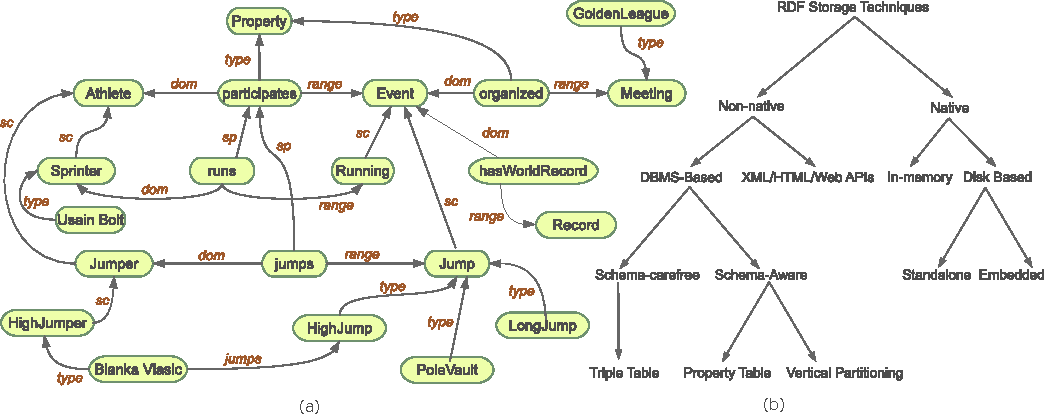
\includegraphics[width=1\textwidth-4pt,%
		bgcolor=white,%
		cfbox=lightestgray % color
			  2pt % rule width
			  0pt % rule separation
			  0pt % margin
	]{images/chapter2/FayeCureBlin2012page5and8.pdf}%
	\caption[RDF graphs]{RDF graphs. (a) An RDF graph describing athletics competitions. (b) A classification of RDF data storage approaches.\sfcite{FayeCureBlin2012}}%
	\label{fig:FayeCureBlin2012page5and8}%
\end{figure}%

RDF is supported by a variety of serialization formats, such as:
\setlist{nolistsep} \begin{itemize}[noitemsep]
	\item RDF/XML,
	\item Turtle,
	\item JSON-LD,
	\item N-Triples,
	\item N3,
	\item N-Quads.
\end{itemize}
They are all human-readable and easy-to-parse.
Some even allow the encoding of inference rules.
In the example shown in \hyperref[code:RDFstoragetechniquesexample]{\autoref{code:RDFstoragetechniquesexample}} is brought how RDF triples may be encoded using the RDF/XML format.
One of the existing ontologies (see the next paragraph for more on Ontologies) is used in the example, that is \texttt{FOAF} (Friend Of A Friend).
FOAF was written to describe people, their activities, and their relationships to other people and objects.\sfcite{FayeCureBlin2012}

\noindent\begin{minipage}{\linewidth} % Wraps the lstlisting inside a minipage of width \linewidth with no indentation to prevent it from splitting between pages
	\lstinputlisting[
		%linerange = {1-29}, % choose line numbers to include
		language = XML,
		mathescape = true,
		label = {code:RDFstoragetechniquesexample},
		caption = {[RDF storage techniques example]RDF storage techniques example}
	]{code/rdfstoragetechniquesexample.xml}
\end{minipage}

The example presents a situation in which there are three vertices of type Person, one of which is named Mark, one is named John, and the third of them is named Peter.
Mark has an email address, while Peter has an RDF description for itself.
Furthermore, Mark knows John and Peter knows Mark.
\medskip

Returning on RDF graphs known as triples stores, some triples stores have been developed as database engines from scratch.
Others, on the other hand, have been developed on top of commercial relational database engines or NoSQL document-oriented database engines already in use.
This method of using existing databases allows for the creation of database engines with minimal programming work.
However, while triples may be stored in relational databases, implementing efficient querying mechanisms (e.g., mapping from SPARQL) into SQL queries for data domains made up of triples is difficult.
As a result, a well-designed native triples store may provide better performance than non-native alternatives.\sfcite{WikipediaTriplestore2021}
\par
\paragraph{Ontologies}\label{paragraph:LiteratureReview/ReviewofGraphDatabaseSystems/Graphdatamodels/RDFgraphsOntologiesInferencesSPARQLSemanticWebandLinkedData/Ontologies}\mbox{}\\\indent
\begin{definition}[of ontologies, vocabularies]\label{definition:ofontologiesvocabularies}
	Because RDF uses URIs to encode information, concepts become more than just words on a page.
	They are linked to a unique definition that anybody can locate on the Web.
	Ontology or vocabulary is the term for this type of shared definition.
\end{definition}

\begin{quoting}[
	begintext={},
	endtext={ - \citeauthor{BernersLeeHendlerLassila2001} in \citetitle{BernersLeeHendlerLassila2001} (\citeyear{BernersLeeHendlerLassila2001})\sfcite{BernersLeeHendlerLassila2001}}
]
	\textit{
		"Imagine having access to a variety of databases with information about people, including their addresses.
		If there was an interest in finding the people living in a specific zip code, it would be required to know which fields in each database represent names and which represent zip codes.
		RDF can specify that '(field 5 in database A) (is a field of type) (zip code)', using URIs rather than phrases for each term.
		However, two databases may use different identifiers for what is in fact the same concept, such as zip code.
		A program that wants to compare or combine information across the two databases has to know that these two terms are being used to mean the same thing.
		Ideally, the program must have a way to discover such common meanings for whatever databases it encounters.
		A solution to this problem is provided by the third basic component of the Semantic Web, collections of information called ontologies."
	}
\end{quoting}

These ontologies (or vocabularies) are thus one of RDF's most distinguishing features.
Ontologies' primary role is to help data integration when there are ambiguities between the terminology used in different datasets, or when a little extra information can lead to the identification of new relationships.
The other role of ontologies is to organize knowledge, which may come from multiple organizations' datasets, in order to disseminate standard and shared terminology.\sfcite{W3CSemanticWebOntologies2021}
\par
\paragraph{Inferences}\mbox{}\\\indent
The possibility to perform inferences (or reasoning) among data is another significant feature of RDF.

\begin{definition}[of inferences]\label{definition:ofinferences}
	Inference is the ability to generate, using by inference engines (or "reasoners") automated procedures - new associations based on data and some additional information in the form of an ontology.
	The new resulting relationships can be returned at query time or explicitly added to the dataset.\sfcite{W3CSemanticWebInference2021}
	This way, in addition to retrieving data, the database can also be used to deduce new information by analyzing facts in the data.
\end{definition}

Inferences, by automatically identifying new relationships while evaluating the data's content, can be used to enhance the quality of data integration on the Web or to manage knowledge on the Web in general.
Inference-based approaches are also useful for detecting inconsistencies in the (integrated) data.\sfcite{W3CSemanticWebInference2021}

Consider the following classical syllogism as an illustration of what inferences are:
Imagine the information:
\begin{quoting}[begintext={}, endtext={}]
	\centering\textit{"all men are mortal"}
\end{quoting}
and
\begin{quoting}[
	begintext={},
	endtext={}
]
	\centering\textit{"Socrates is a man"}
\end{quoting}
is encoded in the RDF graph.
The following conclusion may thus be drawn:
\begin{quoting}[begintext={}, endtext={}]
	\centering\textit{"Socrates is mortal."}
\end{quoting}
This is important when working with entities that belong to classes and subclasses; in fact, inferences would make the fact that a record belonging to a subclass also belongs to its superclass relevant.
This is useful when working with entities that belong to classes and subclasses.
In fact, inferences would consider relevant the fact that a record belonging to a subclass also belongs to its superclass.
The ability to infer is provided by rules specified on metadata, which can be stored with the data itself.
They are usually expressed in OWL (Web Ontology Language), which provides the ability to express notions like:
\setlist{nolistsep} \begin{itemize}[noitemsep]
	\item equality, e.g. \textit{sameAs};
	\item class relationships, e.g. \textit{disjointWith};
	\item richer properties, e.g. \textit{symmetrical};
	\item class property restrictions, e.g. \textit{allValuesFrom}.\sfcite{Lovinger2009}
\end{itemize}

It is therefore commonly used by applications that traverse the graph and must deal with issues that occur when using many different data sources.\sfcite{W3COWLWebOntologyLanguage2004}

Considering another well-known example:
\begin{quoting}[begintext={}, endtext={}]
	\centering\textit{"Epimenides says that all Cretans are liars"}
\end{quoting}
and
\begin{quoting}[begintext={}, endtext={}]
	\centering\textit{"Epimenides is a Cretan"}
\end{quoting}
If the database is programmed to avoid infinite loops, it may point out that there is a contradiction in the data.
Other graph databases usually do not handle such cases by default.\sfcite{Bloor2015}
Nevertheless, some libraries and frameworks are moving in this direction - see \citetitle{ApacheTinkerPopWebsite2021}, \citeauthor{ApacheTinkerPopWebsite2021} (\citeyear{ApacheTinkerPopWebsite2021})\sfcite{ApacheTinkerPopWebsite2021}.

Computers, in order for the semantic web to "work" must have access to structured collections of information and sets of inference rules that they may employ to conduct automated 'reasoning'.
As a result, one of the Semantic Web's challenges has been to provide a language that conveys both data and reasoning rules, as well as the ability to export rules onto the Web from any currently existing knowledge representation system.\sfcite{BernersLeeHendlerLassila2001}
\par
\paragraph{SPARQL}\mbox{}\\\indent
\begin{definition}[of SPARQL]\label{definition:ofSPARQL}
	SPARQL, pronounced as "sparkle"\sfcite{BeckettSPARQL2011} (in IPA phonetic transcription:
	\textnormal{\texttt{/\textprimstress sp\textscripta:kl/}}), is a recursive acronym for "SPARQL Protocol And RDF Query Language".
	It is an RDF query language, i.e. a semantic query language for databases able to retrieve and manipulate data stored in Resource Description Framework (RDF) format.\sfcite{WikipediaSPARQL2021}
\end{definition}

It is not the only RDF query language that exists, but it is the W3C Recommendation in that regard.

SPARQL can express queries on data stored in RDF format natively as well as data viewed in RDF format via middleware.
It supports aggregation, subqueries, negation and limitation on the query by RDF source graph.
SPARQL query results can provide result sets or RDF graphs.\sfcite{W3CSPARQL2008}

(Triple) patterns are the basis for SPARQL searches.
The only difference between triple patterns and RDF triples is that one or more of the constituent resource references are variables.
All triples that meet the patterns are returned by a SPARQL engine.

The following is an example of a query that asks for John's friends:

\noindent\begin{minipage}{1\linewidth} % Wraps the lstlisting inside a minipage of width \linewidth with no indentation to prevent it from splitting between pages
	\lstinputlisting[
		%linerange = {1-29}, % choose line numbers to include
		language = SPARQL,
		mathescape = true,
		label = {code:SPARQLqueryJohnsfriends},
		caption = {[SPARQL query asking for John's friends]SPARQL query asking for John's friends}
	]{code/SPARQLqueryJohnsfriends.sparql}
\end{minipage}

The Semantic Web, an expanded version of the actual Web is possible by the combination of the RDF standard format for data and the SPARQL standard query language.\sfcite{Sinico2017}
\par
\paragraph{Semantic Web and Linked Data}\mbox{}\\\indent
The key notion of Semantic Web can be summarized in these words:
\begin{quoting}[
	begintext={},
	endtext={ - Tim Berners-Lee\sfcite{BernersLeeHendlerLassila2001} referring to the Semantic Web}
]
	\textit{"A new form of Web content that is meaningful to computers"}
\end{quoting}

The Semantic Web is an effort to:
\setlist{nolistsep} \begin{itemize}[noitemsep]
	\item give meaning to web page content;
	\item to enable guided exploration of the contents through the introduction of semantic information;
	\item to provide better processing support for other types of data, aside from web page documents, such as media and structured data;
	\item and more broadly, to provide a means of integrating disparate sources of information.\sfcite{W3CSPARQL2008}
\end{itemize}

The term \textit{Linked Data} refers to a set of guidelines for publishing and linking structured data on the Internet.\sfcite{LinkedData2019}
To make the Web of Data a reality, both nodes and relationships must be published on the Internet, allowing inbound and outbound connections and connecting the local graph to other graphs.

Semantic Web technologies can be used for a wide range of applications, such as:
\setlist{nolistsep} \begin{itemize}[noitemsep]
	\item in resource discovery and classification, to improve domain-specific search engine capabilities;
	\item by intelligent software agents to facilitate knowledge sharing and exchange;
	\item in cataloging to describe the content and content relationships available at a Web site, page, or digital library;
	\item for describing collections of pages that represent a single logical "document";
	\item for content rating;
	\item for describing intellectual property rights of Web pages;
	\item in data integration, where data from multiple sources and formats can be combined into one;
	\item and in many others.\sfcite{W3CHermanRdfFAQ2021}
\end{itemize}

DBPedia, which effectively makes Wikipedia available in RDF, is one example of a large Linked Dataset.
The importance of DBPedia is not just because it contains Wikipedia data, but also because it provides linkages to other Web databases, such as Geonames.
Applications may exploit the extra knowledge from other datasets by using those extra links (in terms of RDF triples).\sfcite{W3CSemanticWebLinkedData2021}
\par
\subsubsection{Hypergraph} \label{subsubsection:LiteratureReview/ReviewofGraphDatabaseSystems/Graphdatamodels/Hypergraph}
A hypergraph is another way to describe graph data.
When datasets contain a high number of many-to-many relationships, hypergraphs can be useful.
However, with hyperedges might be not easy to define fine-grained edge characteristics for the relationships.\sfcite{Sinico2017}

Hypergraph models are more generic than property graphs due to the multi-dimensionality of their hyperedges.
However, because the two are isomorphic, a hypergraph may always be represented as a property graph (albeit with more relationships and nodes).
The opposite, on the other hand, is not so immediate and depends on the information stored.\sfcite{SasakiNeo4j2018}

While property graphs are widely regarded as having the finest combination of pragmatism and modeling efficiency, hypergraphs stand out for their ability to capture meta-intent.
Hypergraphs, for example, need fewer primitives than property graphs when qualifying one connection with another, like in\sfcite{RobinsonWebberEifrem2015}:
\begin{quoting}[begintext={}, endtext={}]
	\centering\textit{"I like the fact that you loved that automobile"}
\end{quoting}

The hypergraph data model did not gain as much traction as the other two data models discussed in the previous subsubsections and only a few graph DBMSs use it to manage data.
HypergraphDB is one example.\sfcite{KobrixHypergraphDB2010}

\subsection{Graph database characteristics} \label{subsection:LiteratureReview/ReviewofGraphDatabaseSystems/Graphdatabasecharacteristics}
Graph databases can be considered from two points of view:
\setlist{nolistsep} \begin{itemize}[noitemsep]
	\item the underlying storage mechanism according which they organize and store graph data,
	\item the processing engine, which itself can be divided:
		\setlist{nolistsep} \begin{itemize}[noitemsep]
			\item with index-free adjacency,
			\item without index-free adjacency.
		\end{itemize}
\end{itemize}

\begin{figure}[H]%
	\centering%
	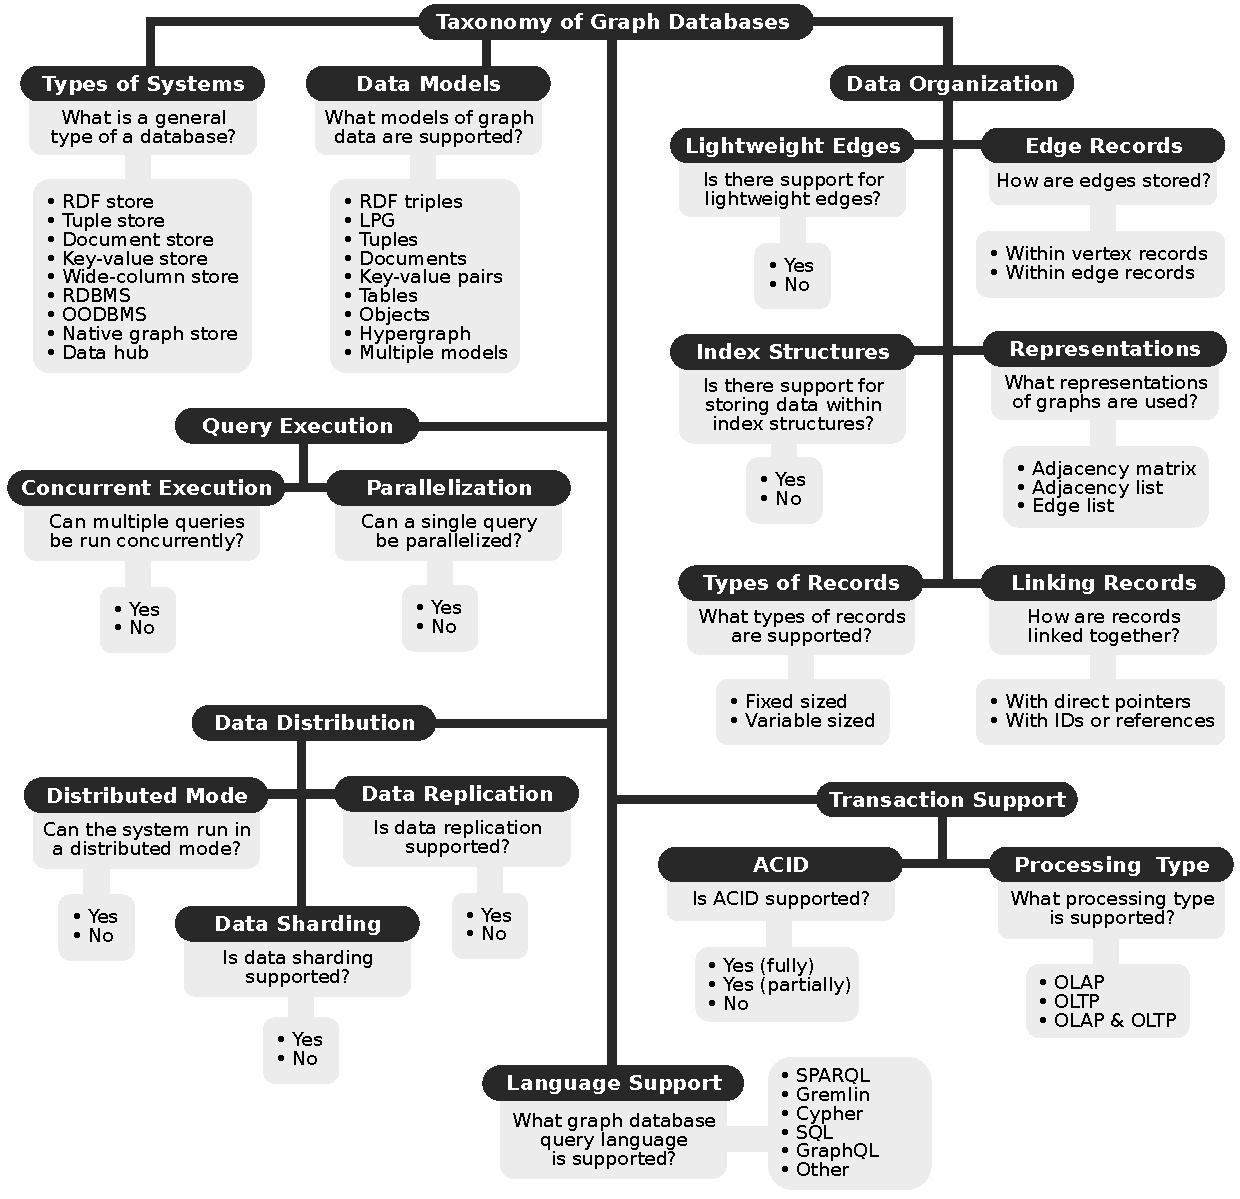
\includegraphics[width=1\textwidth,%
	]{images/chapter2/BestaPeterGerstenbergerFischerPodstawskiBarthelsAlonsoHoefler2019taxonomypage12.pdf}%
	\caption[Taxonomy of Graph Databases]{Taxonomy of Graph Databases\sfcite{BestaPeterGerstenbergerFischerPodstawskiBarthelsAlonsoHoefler2019}}%
	\label{fig:BestaPeterGerstenbergerFischerPodstawskiBarthelsAlonsoHoefler2019taxonomypage12}%
\end{figure}%

From the perspective of the underlying storage mechanism:
\begin{definition}[of native and non-native graph storages]\label{definition:ofnativeandnonnativegraphstorages}
	A graph database is said to be a \textit{native graph storage} if it organizes and stores graph data with an expressly built graph model architecture.
	It is said to be a \textit{non-native graph storage} if it stores graph data with some already existing technology (e.g. relations for a relational database, files, documents, etc).
\end{definition}

Whereas from the perspective of the processing engine, whether they provide or not index-free adjacency:
\begin{definition}[of native and non-native graph processing engine]\label{definition:ofnativeandnonnativegraphprocessingengine}
	A graph database is said to be a \textit{native graph processing engine} if it provides index-free adjacency;
	otherwise it is said to be a \textit{non-native graph processing engine}.
\end{definition}

In a database engine with index-free adjacency, each vertex stores references to its adjacent vertex or of the edges through which the adjacent vertices are reachable.
As a result of this, each vertex serves as a "micro-index" of nearby vertices.
Therefore this approach is in contrast with any system that relies on indexes to discover relations among data and is bound to the \textit{locality principle} of graph queries.
The locality principle says that, for non global graph analytics, during a standard querying only the part of the graph that is reachable by the specified node has to be examined.\sfcite{Sinico2017}

Wanting to evaluate the potential advantages of an index-free adjacency approach:
Assuming a query starts with a specific node.
The aim is to find the descendants of that node that have a specific attribute value.
Assuming that the database that stores such data uses a traditional binary tree index.
If the database does not support index-free adjacency, it will take $ O \left(m \log n \right) $ time to traverse the graph, where $ m $ is the number of hops and $ n $ is the total number of nodes indexed in the graph.
On the other hand, the traversal cost in an implementation with index-free adjacency, would only be $ O \left( m \right) $.\sfcite{RobinsonWebberEifrem2015}
This happens because the information about the edges is already stored in each node - and because the cost to find and traverse each connected edge is $ O \left( 1 \right) $.

This is the common rationale given by the graph databases that support it within their engine.
This motivation however, is as valid as the assumption that traditional databases with no index-free adjacency implement indexes with an algorithmic complexity of $ O \left( \log n \right) $, such as the ones with a binary tree structure.
If a Hash index were to be used, the lookup complexity would be $ O \left( 1 \right) $.
Should be said the one drawback of Hash indexes, is that while exhibiting good performance for direct text matching, they cannot be directly used for partial text matching or range searches.\sfcite{Sinico2017}

There is some disagreement among different graph database product providers on whether a database system must make use of index-free adjacency to be considered a graph database;
For further details on this, see \citetitle{ArangoDBWeinbergerIndexFree2016} - \citeauthor{ArangoDBWeinbergerIndexFree2016} (\citeyear{ArangoDBWeinbergerIndexFree2016}).\sfcite{ArangoDBWeinbergerIndexFree2016}

\subsubsection{Motivations for the adoption of graph databases} \label{subsubsection:LiteratureReview/ReviewofGraphDatabaseSystems/Graphdatabasecharacteristics/Motivationsfortheadoptionofgraphdatabases}
It should be clear by now that graph databases are a useful instrument when the real-world data to be modeled can be described with a graph-like structure and when the required properties are persistence and reliability.

\begin{quoting}[
	begintext={},
	endtext={ - Neo4j's introduction line}
]
	\textit{
		"We live in a connected world.
		There are no isolated pieces of information, but rich, connected domains all around us.
		Only a database that embraces relationships as a core aspect of its data model is able to store, process and query connections efficiently."
	}
\end{quoting}

The more connected the data domain is, the more real value it derives through the relationships.
\gls{Facebook}, was founded on the premise that while discrete information about individuals - their names, what they do, etc. - is valuable, the relationships between them are far more valuable.
Similarly, Larry Page and Sergey Brin figured out not only how to store and analyze discrete online documents, but also how those web documents are linked:
\gls{Google} captured the web graph.\sfcite{RobinsonWebberEifrem2015}

Social graphs, business relationships, recommendation systems, geospatial applications (road maps and route planning for also rail or logistical networks), dependencies (network impact analysis), telecommunication or energy distribution networks, management of distributed data sources and access management are all common use cases for graph databases.\sfcite{Amazon2021, RobinsonWebberEifrem2015}

Fraud detection is another area where graph databases have had a lot of success.
This is accomplished by identifying unusual or properly fraudulent relationship patterns on a graph.
Patterns that deviate from the norm for a particular user can be identified on the graph and reported for further investigation.

In the following paragraphs will be presented a short explanation of the reasons why businesses consider the adoption of graph databases.

\paragraph{Performance}\mbox{}\\\indent
The hoped-for performance boost when working with related data is one reason why businesses look for and choose a graph database.
This is due to the ability to retrieve the vertices that contain only certain types of incoming edges and not others;
or the built-in features to work with weighted graphs and compute shortest or least-cost paths.
The locality principle of graph queries, which was presented in \hyperref[subsection:LiteratureReview/ReviewofGraphDatabaseSystems/Graphdatabasecharacteristics]{\S\ \ref{subsection:LiteratureReview/ReviewofGraphDatabaseSystems/Graphdatabasecharacteristics} - \nameref{subsection:LiteratureReview/ReviewofGraphDatabaseSystems/Graphdatabasecharacteristics}}, contributes to better performance thus making graph database more appetible to businesses.\sfcite{Sinico2017}
\par
\paragraph{Scalability}\mbox{}\\\indent
\begin{figure}[H]%
	\centering%
	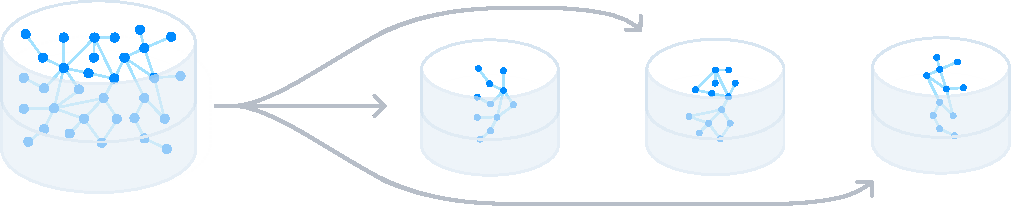
\includegraphics[width=1\textwidth,%
	]{images/chapter2/shardingneo4j.pdf}%
	\caption[Graph database sharding]{Graph database sharding\sfcite{Neo4jGuideDataModeling2021}}%
	\label{fig:shardingneo4j}%
\end{figure}%

Some graph databases provide horizontal scalability at the data level, allowing large graphs to be saved as one across several devices.
Horizontal scalability can help save on hardware, but in graphs comes with higher complexity of setup.
\par
\paragraph{Developer agility and schema flexibility}\mbox{}\\\indent
New types of relationships, vertices, labels and, in general, subgraphs can be added to an existing structure without disrupting existing searches and application functionality.
These factors may have beneficial effects on developer productivity and project maintenance.
Because of the graph model's flexibility, it is not necessary to represent the domain in great detail ahead of time in order to limit future modifications, both in terms of structure (connection types, labels) and vertex and relationship attributes.
Furthermore, the graph data model's schema-free nature eliminates the need for the relational world's schema-oriented data governance operations.\sfcite{RobinsonWebberEifrem2015}

However, this does not imply that schema flexibility is only beneficial; it may also bring problems later in the database life cycle.
\par
\paragraph{Intuitive data model}\mbox{}\\\indent
Both users and developers are comfortable with and intuitive with graphs, and a well-designed query language or \acrshort{API} saves time in both data model definition, development and maintenance.
\par
\subsubsection{Differences from graph computing engines} \label{subsubsection:LiteratureReview/ReviewofGraphDatabaseSystems/Graphdatabasecharacteristics/Differencesfromgraphcomputingengines}
Graph databases and graph computing engines are the two major types of graph data systems.
\setlist{nolistsep} \begin{itemize}[noitemsep]
	\item Graph databases, as described so far, are technologies that are largely used for transactional online graph persistence and are often accessed directly in real time from applications.
	They are the equivalent of the OLTP databases of the relational world.
	\item Graph computing engines (also known as graph analytics engines) are technologies that are largely used for offline graph analytics, which is often done in batches.
	These fall under the same category as other technologies for large-scale data analysis, such as data mining and online analytical processing (OLAP).
	Graph computing engines typically operate on a global graph level and make use of numerous processors to complete batch tasks.\sfcite{AnglesGutierrez2018, RobinsonWebberEifrem2015}
\end{itemize}

Graph computing engines are used to do tasks such as data clustering, like community detection or to answer questions like "how many relationships does anyone in a social network have on average?"
While some graph analytics engines incorporate a graph storage layer, others (and likely the majority) focus solely on processing data from an external source and then deliver the results to store elsewhere.\sfcite{RobinsonWebberEifrem2015}

In some circumstances, graph databases are not the best tool for graph analytics tasks.
The majority of graph processing use random data access.
Random disk access becomes a performance bottleneck for huge graphs that cannot be stored in memory.
Even for smaller graphs that might be entirely kept in memory, graph databases lack the computational capability of distributed and parallel systems since they are centralized systems that must ensure ACID features.
When some computations must be performed on the complete graph in a single-thread technique, computation times quickly become prohibitive.
The implementation of batch processes that conduct several queries with graph-local scope on the database and then do various computations on the intermediate results in order to obtain the graph global result might be one method for computing graph analytics using graph databases.\sfcite{Sinico2017}

The following are some products that perform distributed computation operations:
\setlist{nolistsep} \begin{itemize}[noitemsep]
	\item \textbf{Apache Hadoop} is an open source distributed-processing framework for large data sets.
	It includes a \texttt{MapReduce} implementation.
	Commodity computer clusters can be programmed to execute large-scale data processing in a single pass using Hadoop and \texttt{MapReduce}.
	\texttt{MapReduce} is designed for analytics on big data volumes distributed over hundreds of machines.\sfcite{Sakr2013, DeanGhemawat2008}
	\item \textbf{\gls{Pregel}} is a scalable framework for implementing graph algorithms that was introduced by Google in 2010.
	Graphs, in particular, are intrinsically recursive data structures because vertices' properties are dependent on the qualities of their neighbors, who are dependent on the properties of their neighbors.
	As a result, many important \gls{Pregel} graph algorithms recompute the properties of each vertex iteratively until a fixed-point condition is reached.\sfcite{ApacheSparkGraphX2021, RobinsonWebberEifrem2015}
	\item \textbf{GraphX} is an Apache Spark-based distributed graph processing framework.
	It provides \acrshort{API}s for implementing massively parallel algorithms, like PageRank.
	GraphX fully supports property graphs and is part of Apache Spark.\sfcite{WikipediaApacheSpark2021}
\end{itemize}

\subsubsection{Differences from relational databases} \label{subsubsection:LiteratureReview/ReviewofGraphDatabaseSystems/Graphdatabasecharacteristics/Differencesfromrelationaldatabases}
Relational databases were created with the intent of encoding tabular structures, and they excel at it.
They may, however, struggle to simulate the web of relationships that emerge in various domains of the real world.
One of the strongest arguments for graph databases is:
\begin{quoting}[begintext={}, endtext={}]
	\centering\textit{"Relationships are first-class citizens of the graph data model"}
\end{quoting}
Graph databases do, in fact, value both vertices and relationships equally, storing them with dedicated constructs.
Relationships are the fundamental descriptors for the web of connections among the stored elements and they are the primary information carriers for any programs that need to operate with graph data.d to work with graph data. \sfcite{Sinico2017}
This is not the case in other database management systems, particularly relational ones:
there are no dedicated constructs for treating relationship information differently from other forms of information and connections between entities must be inferred by performing join operations on values of fields with referential integrity constraints (like foreign keys);
or by using out-of-band data processing such as \texttt{MapReduce}.\sfcite{RobinsonWebberEifrem2015}

The relational paradigm is "value-based" by definition:
relationships between two separate relations are expressed by the values that exist within both relations' tuples.
Graph databases, on the other hand, do not need to check and link entities by comparing the values of a given property in both of them;
they already have the linking information stored and all of the operations that relational databases and document databases perform at query time are completely avoided.
The database implementation determines how relationships are kept and linked to the vertices.
When considering those that use index-free adjacency, the basic idea is that the node "record" stores a "pointer" (either logical or physical) to the linked nodes;
or it stores a pointer to some relationship object that stores the information of the other vertex involved, as well as any other possible attribute.
By directly storing relationships, the database relieves the system of those operations that can become burdensome such as \texttt{JOINS}, repeated index searches, temporary tables and so on, especially when dealing with huge amounts of data.\sfcite{Sinico2017}

Relationships are not just valued at the storage layer;
they are also treated with full importance at the conceptual layer.
This fact brings up another crucial feature of graph databases:
the dedicated and simpler handling of relationships in any operations that the users or the programs want to execute on the underlying database.
Making the relationship manageable as a standalone object, rather than being indirectly identified as a secondary object by the two vertexes connected by that edge - simplifies its manipulation in terms of:
\setlist{nolistsep} \begin{itemize}[noitemsep]
	\item property updates,
	\item edge removal or construction
	\item and querying.\sfcite{Sinico2017}
\end{itemize}

Another compelling argument for graph databases is:
\begin{quoting}[begintext={}, endtext={}]
	\textit{"The true value of the graph approach becomes evident when one performs searches that are more than one level deep."}
\end{quoting}

Nested JOINs are the most common mean by which SQL performs hierarchical queries.
When querying "two levels deep" in a recursive relationship, the query consists of a \texttt{JOIN} inside the \texttt{FROM} clause of an outer \texttt{SELECT} clause where another \texttt{JOIN} is executed.
This means that for each desired depth level, would be needed a query consisting of many nested \texttt{SELECT} + \texttt{JOIN} statements as the required depth levels to be traversed.
The more levels deep the querying into the network, the more complex and expensive computations become.
Though the question "who are my friends-of-friends-of-friends?" can be answered in a reasonable amount of time, queries with four, five, or six degrees of friendship degrade dramatically due to the computational and space difficulty of recursively linking tables.\sfcite{RobinsonWebberEifrem2015}

Most relational databases provide a way to overcome situations of execution of nested \texttt{JOIN}s on sub-queries by using a special type of CTE (Common Table Expression) that is invoked by the WITH RECURSIVE clause.\sfcite{Sinico2017}

A last distinction between the relational and the graph model is that the separation between schema and data (instances) in graph databases is less pronounced than in relational databases.
The translation between the "conceptual schema" and the "logical schema," which is part of the usual database development process, is typically imperceptible in graph databases.
In contrast, the transformation of an ER schema to a relational "logical schema" is less straightforward.
This is due to the normalization processes that must be applied to the ER schema in order to map it to a relational "logical schema".
Furthermore, such normalization stages frequently tend to push the developer move away from the reality aimed to represent.
Also, often this stage may cause a reduction of performance.
This is also why denormalization steps are sometimes implemented afterwards.\sfcite{AnglesGutierrez2018, Sinico2017}

\subsubsection{Differences from document stores} \label{subsubsection:LiteratureReview/ReviewofGraphDatabaseSystems/Graphdatabasecharacteristics/Differencesfromdocumentstores}
When dealing with graph data, relational databases are not the only ones to struggle.
Most NoSQL databases indeed store sets of disconnected documents, values or columns.
This makes it difficult to use them for connected data and graphs.
In document stores, the simplest way for defining relationships between two document records is by embedding in the outer document, the document which is to be linked.
Hierarchical situations can be represented using this approach;
However it is immediate to see that if more documents are linked to the same document record, then such record would be replicated for both the outer documents;
This would be a problem with many bad side effects.\sfcite{Sinico2017}

Another well-known method for adding relationships in such stores is to embed a record identifier in the other record rather than entirely embedding it.
This way is resolved the issue of duplication of records and foreign keys may be applied.
However, since with this second approach relationships are built from these flat, disconnected data structures, this approach presents the necessity to join records at the application level - which becomes quickly expensive.
In addition, to ensure that the application updates or deletes these foreign record references in the same way that the rest of the data is updated or deleted, certain consistency methods must be provided.
If this were not to happen, the store would accumulate dangling references which lower query performance and data quality.\sfcite{RobinsonWebberEifrem2015}

Another flaw in this method is that there are no reverse directed, backward pointing identifiers;
the foreign "links" are not reflexive - therefore it is not possible to perform queries in the opposite direction.\sfcite{Sinico2017}

\subsection{Graph Query Languages} \label{subsection:LiteratureReview/ReviewofGraphDatabaseSystems/GraphQueryLanguages}
When working with graph databases, the querying is though differently from the traditional relational database style queries.
Instead of reasoning with tables, columns, joins and so on like in "SQL form", the main focus here are nodes and traversing the graph by walking the right edges.\sfcite{RobinsonWebberEifrem2015}

\begin{figure}[H]%
	\centering%
	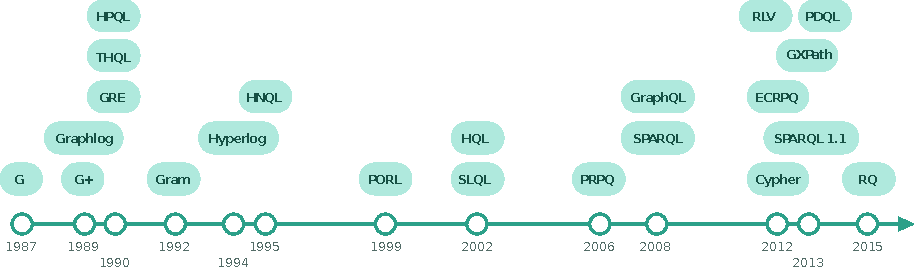
\includegraphics[width=1\textwidth]{images/chapter2/AnglesGutierrez2018graphquerylangpage21.pdf}%
	\caption[Evolution of graph query languages]{Evolution of graph query languages\sfcite{AnglesGutierrez2018}}%
	\label{fig:AnglesGutierrez2018graphquerylangpage21}%
\end{figure}%

Graph queries usually are made of two parts:
\setlist{nolistsep} \begin{enumerate}[noitemsep]
	\item the landing phase,
	\item the exploration phase.
\end{enumerate}

During the landing phase, generally is searched for the start vertex on the graph.
This usually makes use of indices, labels or classes and properties for fast node look-up.
The start node represents the starting point for the exploration phase that shall be performed right-after.
There are situations in which during the landing phase more than one start node is searched.
The same is valid for edges.
On large graphs, the landing phase represents the most expensive operation.
For queries with complex exploration phase, the landing phase could represent a fraction of the total query time.
Following the landing phase is the exploration phase of the querying;
During this phase in a certain sense happens the actual querying, the graph traversal - walking.
The exploration phase makes use of a variety of graph theory navigation algorithms.
The separation of landing and exploratory phase is noticeable also in the query formulation of many graph query languages.
While syntactically this may not be the case in a few languages, their query execution nonetheless follows the same philosophy.\sfcite{Sinico2017}

In the following subsubsections a couple of Graph Query Languages are briefly described.

\subsubsection[Cypher]{Cypher} \label{subsubsection:LiteratureReview/ReviewofGraphDatabaseSystems/GraphQueryLanguages/Cypher}

Cypher\sfcite{Neo4jCypher2021} is a graph query language that is used to conduct graph traversals and Create Retrieve Update Delete (CRUD) operations on the Neo4j graph database.
Cypher is declarative in nature and very expressive in terms of visual and logical representation of graph query patterns and relationship dependencies.\sfcite{SmartM2METSI2020}

\begin{figure}[H]%
	\centering%
	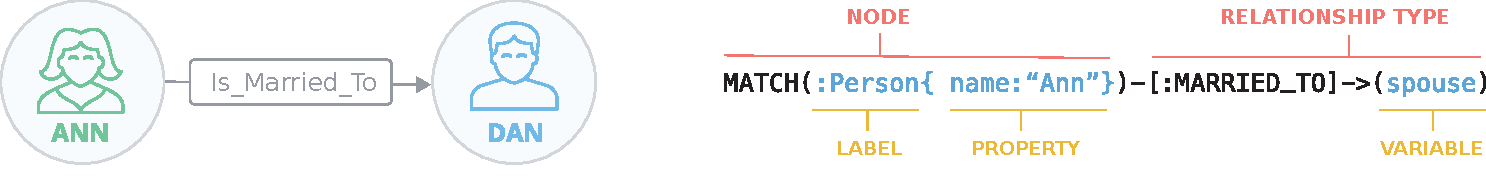
\includegraphics[width=1\textwidth]{images/chapter2/cypher.pdf}%
	\caption[Cypher syntax]{Cypher syntax\sfcite{Neo4jCypher2021}}%
	\label{fig:cypher}%
\end{figure}%

\subsubsection{Gremlin} \label{subsubsection:LiteratureReview/ReviewofGraphDatabaseSystems/GraphQueryLanguages/Gremlin}
Gremlin\sfcite{ApacheTinkerPopGremlin2021, ChanNeubauer2013} is a graph query language that is supported by Apache TinkerPop, a graph framework for different graph databases.
Gremlin is based on Groovy, an OOP language for
Java Platform.
It supports both imperative and declarative queries and both Online Transactional Processing (OLTP) and Online Transactional Processing (OLTP).\sfcite{SmartM2METSI2020}

A Gremlin query example:

\noindent\colorbox{lightestgray}{
	\parbox{1\linewidth-9pt}{%
		\texttt{gremlin> g.V().has('Person', 'name', 'Ann')}
	}%
}%

\noindent\colorbox{lightestgray}{
	\parbox{1\linewidth-9pt}{%
		\texttt{gremlin> valueMap()with(WithOptions.tokens).unfold()}
	}%
}%

\subsubsection[ArangoDB Query Language (AQL)]{ArangoDB Query Language (\acrshort{AQL})} \label{subsubsection:LiteratureReview/ReviewofGraphDatabaseSystems/GraphQueryLanguages/ArangoDBQueryLanguageAQL}
Arango Query Language (\acrshort{AQL}) is used to carry out data modification operations in ArangoDB as well as graph
traversals.
It is a declarative language, written in Java and C.
Because \acrshort{AQL} is used to retrieve all sorts of datasets stored in ArangoDB, it is not limited to graph traversal queries.
\acrshort{AQL} supports the complex query patterns and the different data model (documents, graphs, and key-values). but does not support creating and dropping data entities.
Furthermore, \acrshort{AQL} also supports different traversal functionalities such as searching path using inbound and outbound relationships,
result filtrations, shortest path traversals, community detection and many more \gls{Pregel} custom algorithms.\sfcite{SmartM2METSI2020}

An \acrshort{AQL} query example:

\noindent\colorbox{lightestgray}{
	\parbox{1\linewidth-9pt}{%
		\texttt{FOR p IN Person}
		
		\texttt{\ \ \ \ FILTER p.name == 'Ann'}
		
		\texttt{\ \ \ \ RETURN p}
	}%
}%

\subsubsection{Query Language summary} \label{subsubsection:LiteratureReview/ReviewofGraphDatabaseSystems/GraphQueryLanguages/QueryLanguagesummary}
In \hyperref[longtable:graphquerylanguages]{\autoref{longtable:graphquerylanguages}}\sfcite{SmartM2METSI2020} is brought a summary of the features of the Graph Query Languages presented above.
\begin{center}
	\vspace*{-0.25cm}
	\begin{longtable}{p{0.222\linewidth}p{0.222\linewidth}p{0.222\linewidth}p{0.222\linewidth}}
		\hline \hline
		\textbf{} & \textbf{Cypher} & \textbf{Gremlin} & \textbf{\acrshort{AQL}}\\
		\hline \hline
		\endfirsthead
		
		\multicolumn{4}{l}{... continued from previous page}\\
		\hline \hline
		\textbf{} & \textbf{Cypher} & \textbf{Gremlin} & \textbf{\acrshort{AQL}}\\
		\hline \hline
		\endhead
		
		\hline
		\caption*{\tablename\ \thetable{}: \nameref*{longtable:graphquerylanguages}. Continues on next page ...}
		\vspace*{0.5cm}
		\endfoot
		
		\hline
		%\multicolumn{2}{| c |}{End of Table}\\
		%\hline
		\caption[Feature-wise comparison of selected Graph Query Languages]{Feature-wise comparison of selected Graph Query Languages\sfcite{SmartM2METSI2020}}\label{longtable:graphquerylanguages}
		\vspace*{0.5cm}
		\endlastfoot

		\textbf{Query Language Type} & Declarative & Declarative/Imperative & Declarative/\gls{data manipulation}\\
		\hline
		\textbf{Effort (Query formation)} & Low & Medium & Low\\
		\hline
		\textbf{Readability} & Medium & Low & Medium\\
		\hline
		\textbf{Expressiveness} & High & Medium & High\\
		\hline
		\textbf{Access} & Embedded, WebSocket, REST & Embedded, Websockets, HTTP & REST \& \gls{GraphQL}\\
		\hline
		\textbf{OLTP} & Yes & Yes & Yes\\
		\hline
		\textbf{OLAP} & Yes & Yes & No\\
		\hline
		\textbf{Shortest Path Search} & Yes & Yes & Yes \\
		\hline
	\end{longtable}
	\vspace*{-1.35cm}
\end{center}

\subsection{GDBMSs comparison}\label{subsection:LiteratureReview/ReviewofGraphDatabaseSystems/GDBMSscomparison}
It is possible to find in literature many benchmarking studies carried out in the last years, easily accessible online.
However, it should be noted that the validity of the comparisons of Graph DBMSs is very short since it is a highly in-development field.
A feature of a GDBMS that is not be available in a certain version of the software, might already be implemented in a successive version.
Or viceversa, a feature available in a certain version of the software, might be deprecated in later versions.
Since the changes are rather dynamic, the comparisons are to be taken with a grain of salt.

Furthermore, some of the benchmarking works are made from GDBMS product companies' insiders, or in certain ways related.
Because of this there might also be some bais, cherrypicking in those works.

Below is reported a list of GDBMSs benchmarking works:
\setlist{nolistsep} \begin{itemize}[noitemsep]
	\item \citetitle{BestaPeterGerstenbergerFischerPodstawskiBarthelsAlonsoHoefler2019} - \citeauthor{BestaPeterGerstenbergerFischerPodstawskiBarthelsAlonsoHoefler2019} (\citeyear{BestaPeterGerstenbergerFischerPodstawskiBarthelsAlonsoHoefler2019}) \sfcite{BestaPeterGerstenbergerFischerPodstawskiBarthelsAlonsoHoefler2019}
	\item \citetitle{DayarathnaSuzumura2012} - \citeauthor{DayarathnaSuzumura2012} (\citeyear{DayarathnaSuzumura2012}) \sfcite{DayarathnaSuzumura2012}
	\item \citetitle{CiglanAverbuchHluchy2012} - \citeauthor{CiglanAverbuchHluchy2012} (\citeyear{CiglanAverbuchHluchy2012}) \sfcite{CiglanAverbuchHluchy2012}
	\item \citetitle{BeisPapadopoulosKompatsiaris2015} - \citeauthor{BeisPapadopoulosKompatsiaris2015} (\citeyear{BeisPapadopoulosKompatsiaris2015}) \sfcite{BeisPapadopoulosKompatsiaris2015}
	\item \citetitle{JouiliVansteenberghe2013} - \citeauthor{JouiliVansteenberghe2013} (\citeyear{JouiliVansteenberghe2013}) \sfcite{JouiliVansteenberghe2013}
	\item \citetitle{ArangoDBWeinbergerPerformance2015} \ - \ \citeauthor{ArangoDBWeinbergerPerformance2015} (\citeyear{ArangoDBWeinbergerPerformance2015}) \sfcite{ArangoDBWeinbergerPerformance2015}
	\item \citetitle{W3CRdfStoreBenchmarking2021} - \citeauthor{W3CRdfStoreBenchmarking2021} (\citeyear{W3CRdfStoreBenchmarking2021}) \sfcite{W3CRdfStoreBenchmarking2021}
	\item \citetitle{W3CLargeTripleStores2021} - \citeauthor{W3CLargeTripleStores2021} (\citeyear{W3CLargeTripleStores2021}) \sfcite{W3CLargeTripleStores2021}
	\item Graph vs. Relational comparison: \citetitle{ArangoDBWeinbergerBenchmark2015} - \citeauthor{ArangoDBWeinbergerBenchmark2015} (\citeyear{ArangoDBWeinbergerBenchmark2015}) \sfcite{ArangoDBWeinbergerBenchmark2015}
\end{itemize}

In the next subsubsection, an in-detail view of major Graph DBMSs is given.

\subsubsection{Major Graph DBMSs} \label{subsubsection:LiteratureReview/ReviewofGraphDatabaseSystems/GDBMSscomparison/MajorGraphDBMSs}
Since by now the number of GDBMS products available in the market is of more than 30, doing a hand-by-hand manual analysis of each product continuously each month is not feasible.
A list of the most known DBMSs is ranked monthly by popularity on the website \citeurl{solid2021}\sfcite{solid2021}.
The different products are categorized and there is a category for Graph Database Systems too.

At the beginning of \hyperref[section:LiteratureReview/ReviewofGraphDatabaseSystems]{\S\ \ref{section:LiteratureReview/ReviewofGraphDatabaseSystems}} was presented a chart (see \hyperref[fig:solid2021popularitychange]{\autoref{fig:solid2021popularitychange}}) from 
\citeurl{solid2021}\sfcite{solid2021} showing the trends of popularity growth between the different categories of DBMSs.
While the growth is staggering, Graph DBMSs have still a long way to do till they catch up the relational DBMSs.
In \hyperref[longtable:solid2021alldbmssrank]{\autoref{longtable:solid2021alldbmssrank}} this is evident.

\citeurl{solid2021}\sfcite{solid2021} calculates the popularity score of a system by standardizing and averaging different parameters. The score for each DBMS is obtained using the following parameters\sfcite{Sinico2017}:
\setlist{nolistsep} \begin{itemize}[noitemsep]
	\item The number of times the system has been mentioned on the web, as measured by the number of times it has come up in search engine queries.
	\item Frequency of searches in Google Trends.
	\item Frequency of technical discussions about the system, measured as the number of questions on Stack Overflow and DBA Stack Exchange.
	\item Number of job offers, in which the system is mentioned, on the leading job search engines.
	\item Number of \gls{LinkedIn} and \gls{Upwork} profiles in which the system is mentioned.
	\item Number of \gls{Twitter} tweets in which the system is mentioned.
\end{itemize}

To be noted however, the disclaimer on \citeurl{solid2021}:
\begin{quoting}[
	begintext={},
	endtext={\sfcite{solid2021}}
]
	\textit{
		"Ranking does not measure the number of installations of the systems, or their use within IT systems.
		It can be expected, that an increase in the popularity of a system as measured by the \textnormal{\citeurl{solid2021}} Ranking (e.g. in discussions or job offers) precedes a corresponding broad use of the system by a certain time factor.
		Because of this, the \textnormal{\citeurl{solid2021}} Ranking can act as an early indicator"
	}
\end{quoting}

\begin{center}
	\vspace*{-0.25cm}
	\begin{longtable}{p{1\textwidth-2\tabcolsep}}
		\hspace*{-1\tabcolsep}
		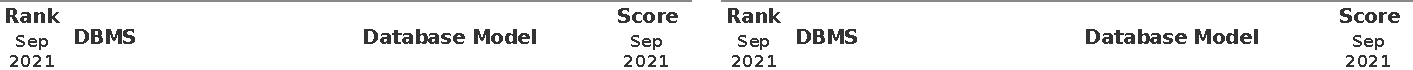
\includegraphics[width=1\textwidth-0.5\tabcolsep]{%
			tables/chapter2/solid2021alldbmssrankheader.pdf%
		}
		\endfirsthead
		
		\multicolumn{1}{l}{... continued from previous page}\\
		\hspace*{-1\tabcolsep}
		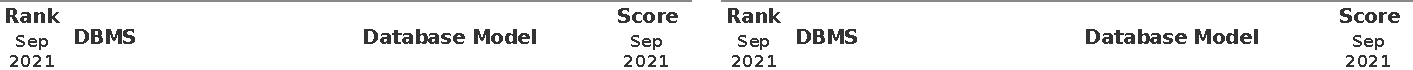
\includegraphics[width=1\textwidth-0.5\tabcolsep]{%
			tables/chapter2/solid2021alldbmssrankheader.pdf%
		}
		\endhead
		
		\caption*{\tablename\ \thetable{}: \nameref*{longtable:solid2021alldbmssrank}\sfcite{solid2021}. Continues on next page ...}
		\vspace*{0.5cm}
		\endfoot
		
		\caption[Rank by popularity of GDBMSs in top 100 DBMSs]{Rank by popularity of GDBMSs in top 100 DBMSs\sfcite{solid2021}}\label{longtable:solid2021alldbmssrank}
		\vspace*{0.5cm}
		\endlastfoot
		
		\hspace*{-1\tabcolsep}
		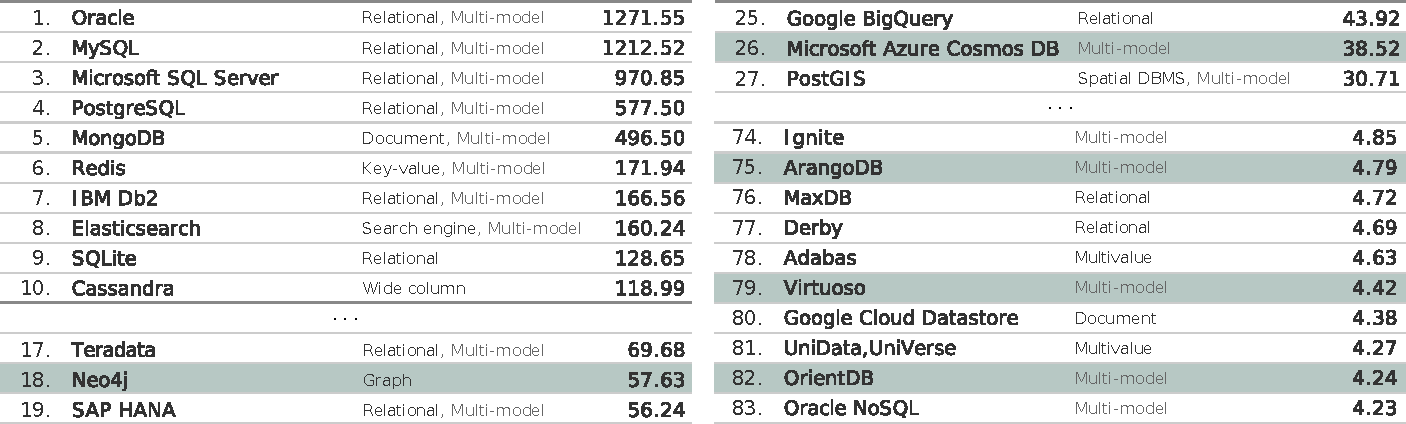
\includegraphics[width=1\textwidth-0.5\tabcolsep]{%
			tables/chapter2/solid2021alldbmssrankrowsnew.pdf%
		}
	\end{longtable}
	\vspace*{-1.35cm}
\end{center}

In \hyperref[fig:solid2021trends]{\autoref{fig:solid2021trends}} is displayed a chart of the trends of selected Graph DBMSs only. Note the score axis in logarithmic scale. At the moment Neo4j is ranked as the most popular Graph Database Management System. It is followed by Microsoft Azure Cosmos Database and ArangoDB.

Whereas in \hyperref[fig:BestaPeterGerstenbergerFischerPodstawskiBarthelsAlonsoHoefler2019categoriespage11]{\autoref{fig:BestaPeterGerstenbergerFischerPodstawskiBarthelsAlonsoHoefler2019categoriespage11}} are reported by \citeauthor{BestaPeterGerstenbergerFischerPodstawskiBarthelsAlonsoHoefler2019} (\citeyear{BestaPeterGerstenbergerFischerPodstawskiBarthelsAlonsoHoefler2019})\sfcite{BestaPeterGerstenbergerFischerPodstawskiBarthelsAlonsoHoefler2019}
the various types of graph database systems with an indication of the data model, way of storing vertices and edges, a drawing of the data structures and examples of which GDBMS belongs to that category.

\begin{figure}[H]%
	\centering%
	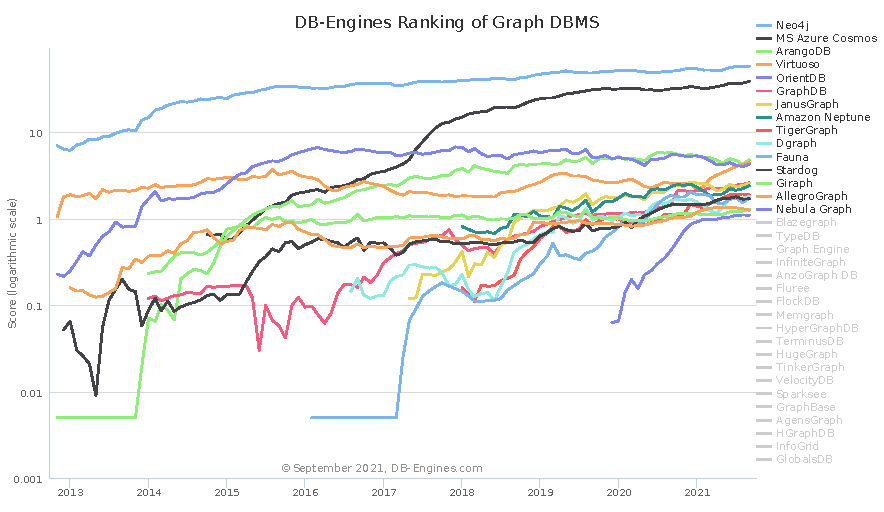
\includegraphics[width=1\textwidth-4pt,%
		bgcolor=white,%
		cfbox=lightestgray % color
			  2pt % rule width
			  0pt % rule separation
			  0pt % margin
	]{images/chapter2/solid2021trends.pdf}%
	\caption[Trend of Graph DBMS Popularity]{Trend of Graph DBMS Popularity\sfcite{solid2021}}%
	\label{fig:solid2021trends}%
\end{figure}%

\begin{figure}[H]%
	\centering%
	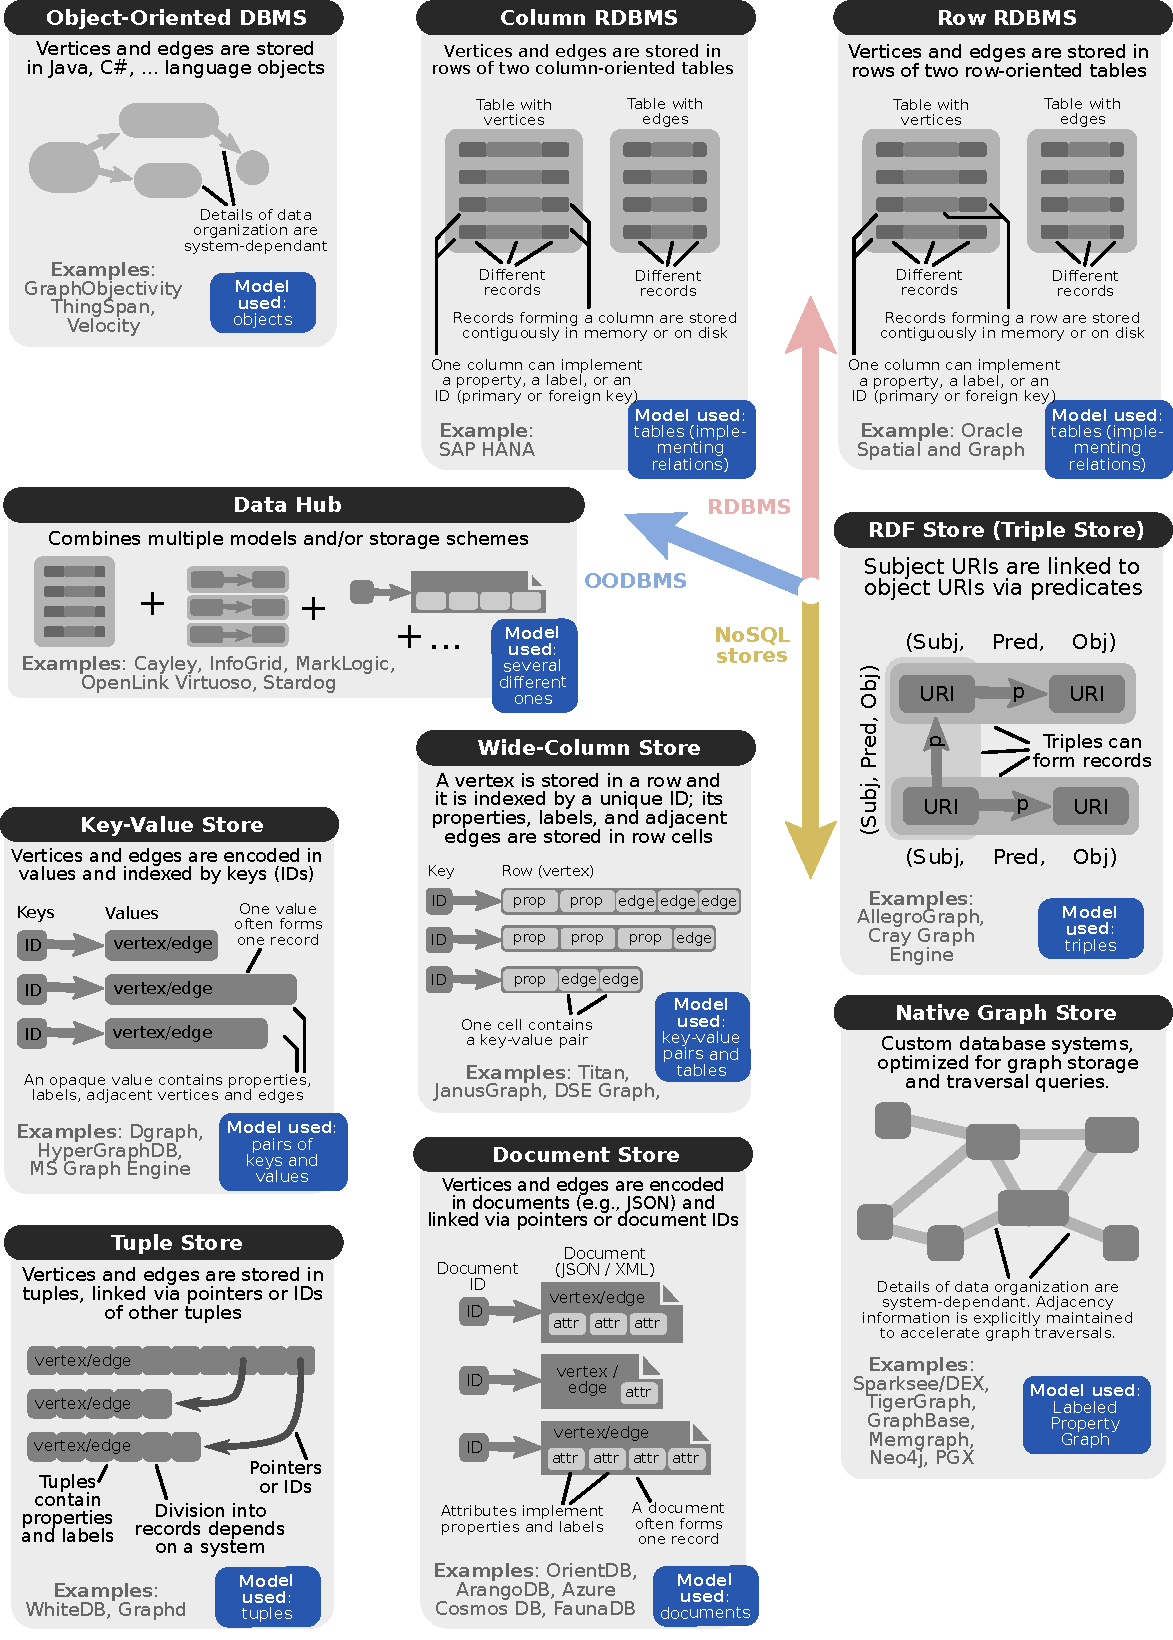
\includegraphics[width=1\textwidth,%
	]{images/chapter2/BestaPeterGerstenbergerFischerPodstawskiBarthelsAlonsoHoefler2019categoriespage11.pdf}%
	\caption[Overview of different categories of graph database systems, with examples]{Overview of different categories of graph database systems, with examples\sfcite{BestaPeterGerstenbergerFischerPodstawskiBarthelsAlonsoHoefler2019}}%
	\label{fig:BestaPeterGerstenbergerFischerPodstawskiBarthelsAlonsoHoefler2019categoriespage11}%
\end{figure}%

In the next subsubsection a comparison of the major GDBMSs summarized in two tables is presented.

\subsubsection{Comparison tables} \label{subsubsection:LiteratureReview/ReviewofGraphDatabaseSystems/GDBMSscomparison/Comparisontables}
In \hyperref[longtable:BestaPeterGerstenbergerFischerPodstawskiBarthelsAlonsoHoefler2019tables]{\autoref{longtable:BestaPeterGerstenbergerFischerPodstawskiBarthelsAlonsoHoefler2019tables}} is brought an exhaustive comparison of all known graph database systems with indications on data models, storing mechanisms, operation mode, kind of transactions and other remarks. The various GDBMSs are divided in categories according to the data model used. To consult the original work, see \citetitle{BestaPeterGerstenbergerFischerPodstawskiBarthelsAlonsoHoefler2019} - \citeauthor{BestaPeterGerstenbergerFischerPodstawskiBarthelsAlonsoHoefler2019} (\citeyear{BestaPeterGerstenbergerFischerPodstawskiBarthelsAlonsoHoefler2019})\sfcite{BestaPeterGerstenbergerFischerPodstawskiBarthelsAlonsoHoefler2019}.

\begin{center}
	\vspace*{-0.25cm}
	\begin{longtable}{p{1\textwidth-2\tabcolsep}}
		\hspace*{-1\tabcolsep}
		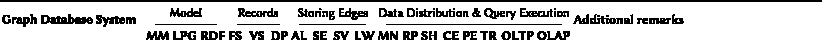
\includegraphics[width=1\textwidth-0.5\tabcolsep]{%
			tables/chapter2/BestaPeterGerstenbergerFischerPodstawskiBarthelsAlonsoHoefler2019tablesheader.pdf%
		}
		\endfirsthead
		
		\multicolumn{1}{l}{... continued from previous page}\\
		\hspace*{-1\tabcolsep}
		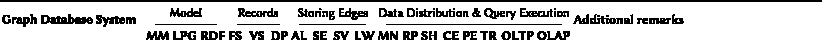
\includegraphics[width=1\textwidth-0.5\tabcolsep]{%
			tables/chapter2/BestaPeterGerstenbergerFischerPodstawskiBarthelsAlonsoHoefler2019tablesheader.pdf%
		}
		\endhead
		
		\hspace*{-1\tabcolsep}
		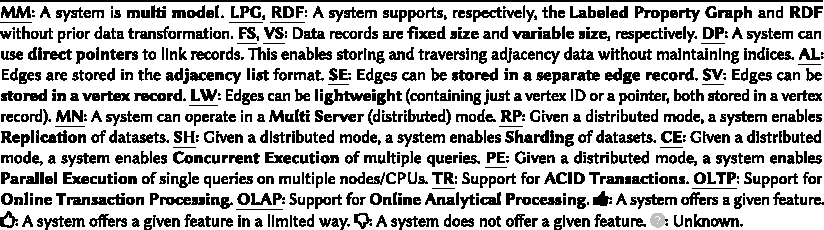
\includegraphics[width=1\textwidth-0.5\tabcolsep]{%
			tables/chapter2/BestaPeterGerstenbergerFischerPodstawskiBarthelsAlonsoHoefler2019tablesfooter.pdf%
		}\\
		\caption*{\tablename\ \thetable{}: \nameref*{longtable:BestaPeterGerstenbergerFischerPodstawskiBarthelsAlonsoHoefler2019tables}\sfcite{BestaPeterGerstenbergerFischerPodstawskiBarthelsAlonsoHoefler2019}. Continues on next page ...}
		\vspace*{0.5cm}
		\endfoot
		
		\hspace*{-1\tabcolsep}
		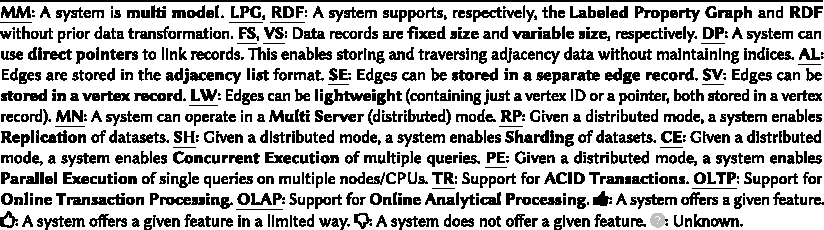
\includegraphics[width=1\textwidth-0.5\tabcolsep]{%
			tables/chapter2/BestaPeterGerstenbergerFischerPodstawskiBarthelsAlonsoHoefler2019tablesfooter.pdf%
		}\\
		\caption[Comparison of graph databases]{Comparison of graph databases\sfcite{BestaPeterGerstenbergerFischerPodstawskiBarthelsAlonsoHoefler2019}}\label{longtable:BestaPeterGerstenbergerFischerPodstawskiBarthelsAlonsoHoefler2019tables}
		\vspace*{0.5cm}
		\endlastfoot
		
		\hspace*{-1\tabcolsep}
		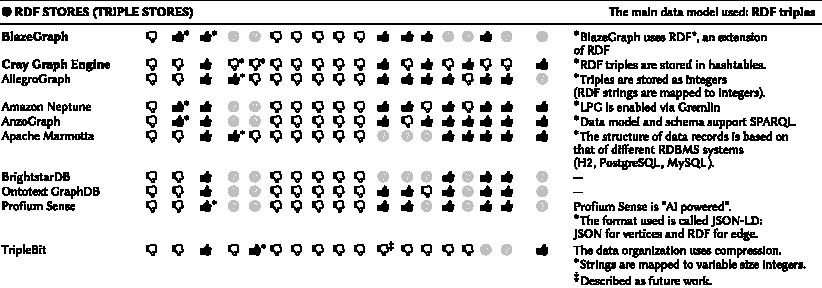
\includegraphics[width=1\textwidth-0.5\tabcolsep]{%
			tables/chapter2/BestaPeterGerstenbergerFischerPodstawskiBarthelsAlonsoHoefler2019tablesrow1.pdf%
		}\\
		\hspace*{-1\tabcolsep}
		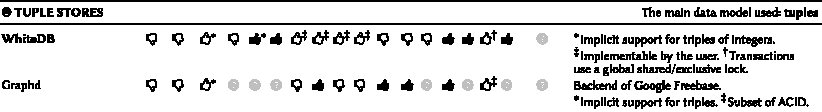
\includegraphics[width=1\textwidth-0.5\tabcolsep]{%
			tables/chapter2/BestaPeterGerstenbergerFischerPodstawskiBarthelsAlonsoHoefler2019tablesrow2.pdf%
		}\\
		\hspace*{-1\tabcolsep}
		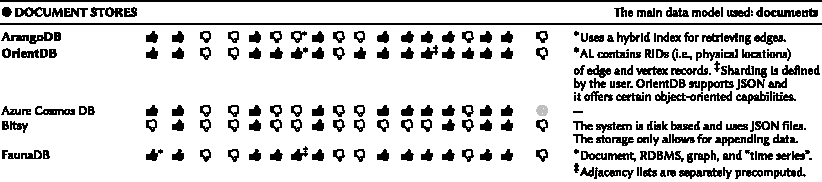
\includegraphics[width=1\textwidth-0.5\tabcolsep]{%
			tables/chapter2/BestaPeterGerstenbergerFischerPodstawskiBarthelsAlonsoHoefler2019tablesrow3.pdf%
		}\\
		\hspace*{-1\tabcolsep}
		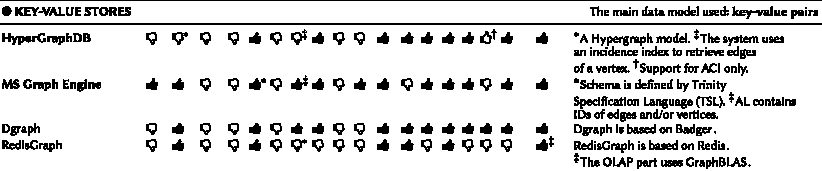
\includegraphics[width=1\textwidth-0.5\tabcolsep]{%
			tables/chapter2/BestaPeterGerstenbergerFischerPodstawskiBarthelsAlonsoHoefler2019tablesrow4.pdf%
		}\\
		\hspace*{-1\tabcolsep}
		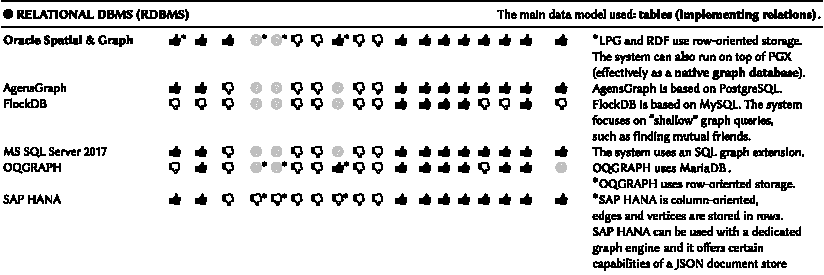
\includegraphics[width=1\textwidth-0.5\tabcolsep]{%
			tables/chapter2/BestaPeterGerstenbergerFischerPodstawskiBarthelsAlonsoHoefler2019tablesrow6.pdf%
		}\\
		\hspace*{-1\tabcolsep}
		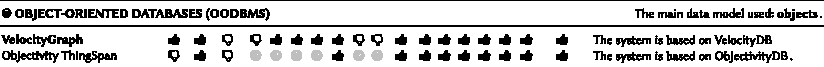
\includegraphics[width=1\textwidth-0.5\tabcolsep]{%
			tables/chapter2/BestaPeterGerstenbergerFischerPodstawskiBarthelsAlonsoHoefler2019tablesrow7.pdf%
		}\\
		\hspace*{-1\tabcolsep}
		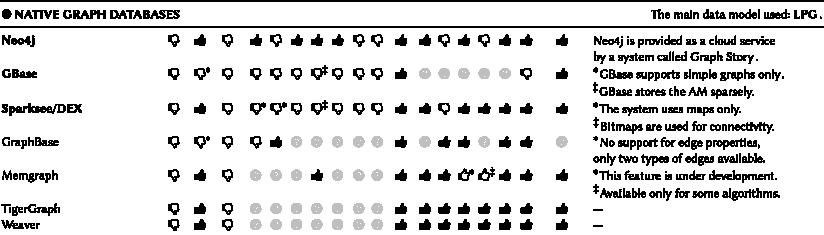
\includegraphics[width=1\textwidth-0.5\tabcolsep]{%
			tables/chapter2/BestaPeterGerstenbergerFischerPodstawskiBarthelsAlonsoHoefler2019tablesrow8.pdf%
		}\\
		\hspace*{-1\tabcolsep}
		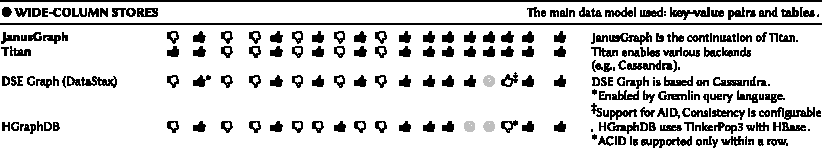
\includegraphics[width=1\textwidth-0.5\tabcolsep]{%
			tables/chapter2/BestaPeterGerstenbergerFischerPodstawskiBarthelsAlonsoHoefler2019tablesrow5.pdf%
		}\\
		\hspace*{-1\tabcolsep}
		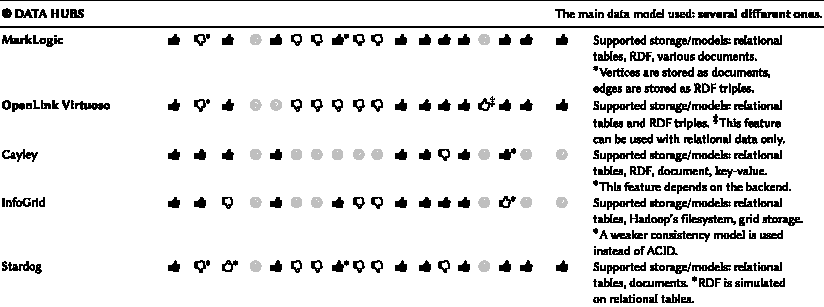
\includegraphics[width=1\textwidth-0.5\tabcolsep]{%
			tables/chapter2/BestaPeterGerstenbergerFischerPodstawskiBarthelsAlonsoHoefler2019tablesrow9.pdf%
		}
	\end{longtable}
	\vspace*{-1.35cm}
\end{center}

In the next table is presented the current state of support for different graph QLs in the various GDBMSs.

\begin{center}
	\vspace*{-0.25cm}
	\begin{longtable}{p{1\textwidth-2\tabcolsep}}
		\hspace*{-1\tabcolsep}
		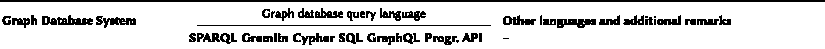
\includegraphics[width=1\textwidth-0.5\tabcolsep]{%
			tables/chapter2/BestaPeterGerstenbergerFischerPodstawskiBarthelsAlonsoHoefler2019tablesQLheader.pdf%
		}
		\endfirsthead
		
		\multicolumn{1}{l}{... continued from previous page}\\
		\hspace*{-1\tabcolsep}
		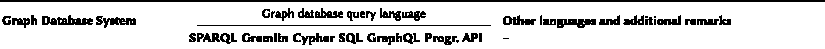
\includegraphics[width=1\textwidth-0.5\tabcolsep]{%
			tables/chapter2/BestaPeterGerstenbergerFischerPodstawskiBarthelsAlonsoHoefler2019tablesQLheader.pdf%
		}
		\endhead
		
		\hspace*{-1\tabcolsep}
		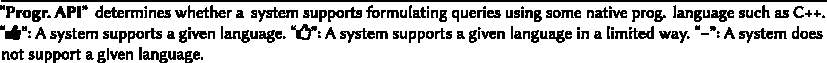
\includegraphics[width=1\textwidth-0.5\tabcolsep]{%
			tables/chapter2/BestaPeterGerstenbergerFischerPodstawskiBarthelsAlonsoHoefler2019tablesQLfooter.pdf%
		}\\
		\caption*{\tablename\ \thetable{}: \nameref*{longtable:BestaPeterGerstenbergerFischerPodstawskiBarthelsAlonsoHoefler2019tablesQL}\sfcite{BestaPeterGerstenbergerFischerPodstawskiBarthelsAlonsoHoefler2019}. Continues on next page ...}
		\vspace*{0.5cm}
		\endfoot
		
		\hspace*{-1\tabcolsep}
		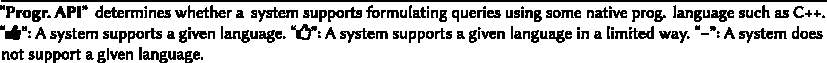
\includegraphics[width=1\textwidth-0.5\tabcolsep]{%
			tables/chapter2/BestaPeterGerstenbergerFischerPodstawskiBarthelsAlonsoHoefler2019tablesQLfooter.pdf%
		}\\
		\caption[Support for different graph query languages in different GDBMSs]{Support for different graph query languages in different GDBMSs\sfcite{BestaPeterGerstenbergerFischerPodstawskiBarthelsAlonsoHoefler2019}}\label{longtable:BestaPeterGerstenbergerFischerPodstawskiBarthelsAlonsoHoefler2019tablesQL}
		\vspace*{0.5cm}
		\endlastfoot
		
		\hspace*{-1\tabcolsep}
		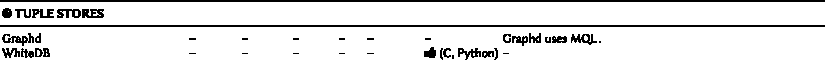
\includegraphics[width=1\textwidth-0.5\tabcolsep]{%
			tables/chapter2/BestaPeterGerstenbergerFischerPodstawskiBarthelsAlonsoHoefler2019tablesQLrow2.pdf%
		}\\
		\hspace*{-1\tabcolsep}
		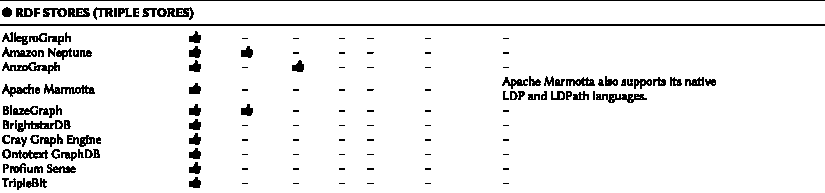
\includegraphics[width=1\textwidth-0.5\tabcolsep]{%
			tables/chapter2/BestaPeterGerstenbergerFischerPodstawskiBarthelsAlonsoHoefler2019tablesQLrow1.pdf%
		}\\
		\hspace*{-1\tabcolsep}
		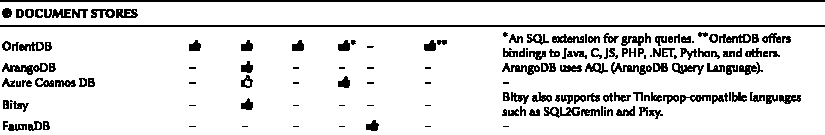
\includegraphics[width=1\textwidth-0.5\tabcolsep]{%
			tables/chapter2/BestaPeterGerstenbergerFischerPodstawskiBarthelsAlonsoHoefler2019tablesQLrow3.pdf%
		}\\
		\hspace*{-1\tabcolsep}
		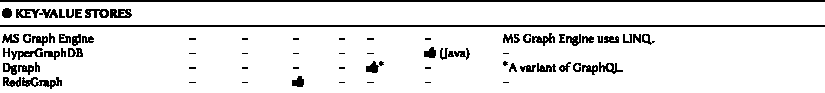
\includegraphics[width=1\textwidth-0.5\tabcolsep]{%
			tables/chapter2/BestaPeterGerstenbergerFischerPodstawskiBarthelsAlonsoHoefler2019tablesQLrow4.pdf%
		}\\
		\hspace*{-1\tabcolsep}
		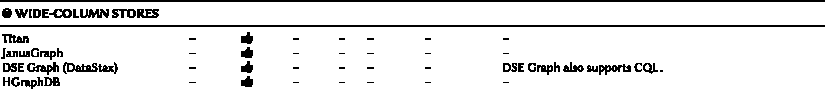
\includegraphics[width=1\textwidth-0.5\tabcolsep]{%
			tables/chapter2/BestaPeterGerstenbergerFischerPodstawskiBarthelsAlonsoHoefler2019tablesQLrow5.pdf%
		}\\
		\hspace*{-1\tabcolsep}
		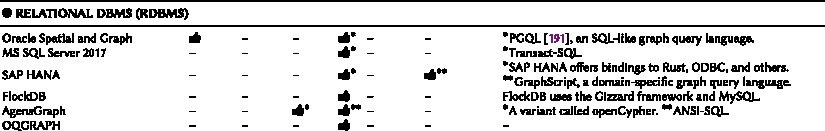
\includegraphics[width=1\textwidth-0.5\tabcolsep]{%
			tables/chapter2/BestaPeterGerstenbergerFischerPodstawskiBarthelsAlonsoHoefler2019tablesQLrow6.pdf%
		}\\
		\hspace*{-1\tabcolsep}
		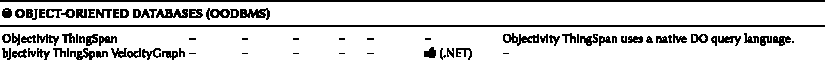
\includegraphics[width=1\textwidth-0.5\tabcolsep]{%
			tables/chapter2/BestaPeterGerstenbergerFischerPodstawskiBarthelsAlonsoHoefler2019tablesQLrow7.pdf%
		}\\
		\hspace*{-1\tabcolsep}
		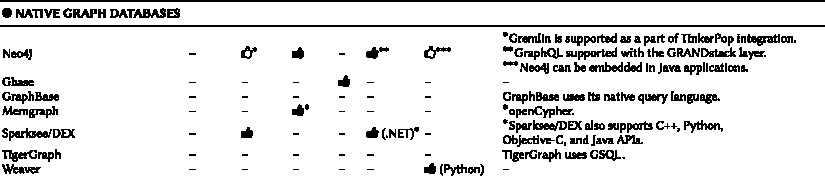
\includegraphics[width=1\textwidth-0.5\tabcolsep]{%
			tables/chapter2/BestaPeterGerstenbergerFischerPodstawskiBarthelsAlonsoHoefler2019tablesQLrow8.pdf%
		}\\
		\hspace*{-1\tabcolsep}
		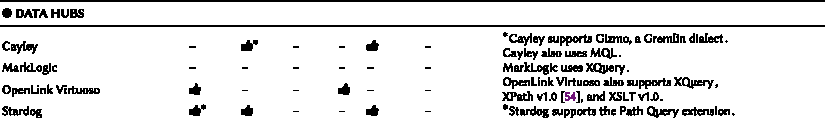
\includegraphics[width=1\textwidth-0.5\tabcolsep]{%
			tables/chapter2/BestaPeterGerstenbergerFischerPodstawskiBarthelsAlonsoHoefler2019tablesQLrow9.pdf%
		}
	\end{longtable}
	\vspace*{-1.35cm}
\end{center}

In the next subsection a GDBMS is taken into consideration, specifically ArangoDB - and its characteristics are presented in detail.

\subsection{A GDBMS in detail: ArangoDB} \label{subsection:LiteratureReview/ReviewofGraphDatabaseSystems/AGDBMSindetailArangoDB}
ArangoDB is a NoSQL multi-model database management system supporting graphs, documents and key/value pairs.
It was first released in 2012 and is developed by ArangoDB GmbH and triAGENS GmbH (Germany).
In September 2021, according to \citeurl{solid2021}\sfcite{solid2021}, it ranks:
\setlist{nolistsep} \begin{itemize}[noitemsep]
	\item \ 3\textsuperscript{rd} in Graph DBMS category,
	\item 10\textsuperscript{th} in Document Stores category,
	\item 11\textsuperscript{th} in Key-Value Stores category,
	\item 75\textsuperscript{th} overall the DBMS tracked by the site.
\end{itemize}

It is a schema-free database management system written in C/C++ and JavaScript that runs on a variety of operating systems (Linux, OS X, Windows, Raspbian and Solaris).
ArangoDB is designed to serve documents to clients.
These documents are sent in JSON format over HTTP.
A REST \acrshort{API} is available to interact with the database system.
A web interface and an interactive shell are also available for accessing the database.\sfcite{Sinico2017}

It works with a variety of programming languages: C\#, Clojure, Dart, Elixir, Erlang, Go, Java, JavaScript, PHP, \gls{Python}, R, Ruby, Rust, Scala and so on - and allows the definition of stored procedures in JavaScript.
Many community integrations and libraries exist for ArangoDB, worth mentioning: Camel, Ecto, Feathers, GORM, \gls{GraphQL}, Gremlin, Hemera, Jakarta NoSQL, Kafka, Laravel, Mirconaut, Pydantic, Symfony2, Testcontainers and many others.
It states to have a native multi-model approach, rather to, say, a graph database implemented as an abstraction layer on top of a document store.
In this approach, when executing queries, it "does not switch" between the models behind the scenes.\sfcite{ArangoDBWhyArangoDB2021}

\subsubsection{Logical data organization}\label{subsubsection:LiteratureReview/ReviewofGraphDatabaseSystems/AGDBMSindetailArangoDB/Logicaldataorganization}
ArangoDB organizes data into databases, collections and documents.
Databases are sets of collections.
Collections are sets of records, which are also known as documents.
To have collection isolation, multiple databases can be defined.
A special database called \texttt{\_system} is always generated by default, it cannot be deleted and it is used as the administration database to execute tasks such as user and collection management.\sfcite{Sinico2017}

Documents can be thought of as rows in a table, while collections are the equivalent of tables in RDBMS.
Because ArangoDB is schema-less, there is no need to define what attributes a collection - and consequently its documents - can have before inserting data;
Instead, each document can have a completely different structure while yet being stored with other documents in the same collection.\sfcite{ArangoDBGettingStarted2021, ArangoDBDataModel2021}

There are two types of collections:
\setlist{nolistsep} \begin{itemize}[noitemsep]
	\item document collections, also used as vertex collections in the context of graphs,
	\item and edge collections.
\end{itemize}
Edge collections also store documents, but they also have two special attributes, \_from and \_to, that are used to form relationships between vertex documents.

Documents follow the JSON standard.
Internally they are stored in a binary format called \texttt{VelocyPack}.
\texttt{VelocyPack} is described in \hyperref[subsubsection:LiteratureReview/ReviewofGraphDatabaseSystems/AGDBMSindetailArangoDB/Physicaldataorganization]{\S\ \ref{subsubsection:LiteratureReview/ReviewofGraphDatabaseSystems/AGDBMSindetailArangoDB/Physicaldataorganization} - \nameref{subsubsection:LiteratureReview/ReviewofGraphDatabaseSystems/AGDBMSindetailArangoDB/Physicaldataorganization}} on \hyperref[subsubsection:LiteratureReview/ReviewofGraphDatabaseSystems/AGDBMSindetailArangoDB/Physicaldataorganization]{page \pageref*{subsubsection:LiteratureReview/ReviewofGraphDatabaseSystems/AGDBMSindetailArangoDB/Physicaldataorganization}}.

A document can have zero or more attributes, each with a value.
A value can be:
\setlist{nolistsep} \begin{itemize}[noitemsep]
	\item an atomic type, such as a number, string, boolean or null;
	\item or a compound type, such as an array;
	\item or an embedded document.
\end{itemize}

Each document has a unique primary key that allows it to be identified both within its collection and across all collections in the same database.
The document handle is formed by the combination of the collection name and the document key.\sfcite{ArangoDBDataModel2021}

Three special attributes are part of every document:
\setlist{nolistsep} \begin{itemize}[noitemsep]
	\item the document handle is saved as a string in \texttt{\_id},
	\item the primary key of the document is stored in \texttt{\_key},
	\item and the document revision is recorded in \texttt{\_rev}.
\end{itemize}
  
When creating a document, the user can provide the value of the key attribute.
However, after the document has been produced, the \texttt{\_id} and \texttt{\_key} values remain immutable, while the rev value is automatically maintained by ArangoDB.\sfcite{ArangoDBDataModel2021}

The direction of an edge depends on the fields \texttt{\_from} and \texttt{\_to}.
It is possible to indicate within a query which direction the edge should be traversed. The possible directions are:
\setlist{nolistsep} \begin{itemize}[noitemsep]
	\item \texttt{OUTBOUND}: \texttt{\_from} $ \rightarrow $ \texttt{\_to};
	\item \texttt{INBOUND}: \texttt{\_from} $ \leftarrow $ \texttt{\_to};
	\item \texttt{ANY}: \texttt{\_from} $ \leftrightarrow $ \texttt{\_to}.\sfcite{ArangoDBGraphs2021}
\end{itemize}

In ArangoDB a named graph is used to define graphs.
To define a graph, the edge collections to include are specified.
The related vertex documents are automatically discovered by the \texttt{\_from} \texttt{\_to} attributes of each of the edge documents.\sfcite{ArangoDBGraphs2021}

\subsubsection{Physical data organization}\label{subsubsection:LiteratureReview/ReviewofGraphDatabaseSystems/AGDBMSindetailArangoDB/Physicaldataorganization}
JSON is ArangoDB's 'default data format.\sfcite{Wiese2015}
It can store a nested JSON object as a data entry inside a collection natively,
So there is no need to unwrap the generated JSON objects for storage and the stored data simply inherits the document's tree structure.\sfcite{AgoubKundeKada2016}

ArangoDB, internally, uses \texttt{VelocyPack}.
\texttt{VelocyPack} is a compact binary format for serialization and storage of documents, query results, and temporarily computed values.\sfcite{ArangoDBVelocityPack2021}
VelocyPack is a (unsigned) byte-oriented serialization format whose values are platform-independent bytes sequences.\sfcite{ArangoDBVelocyPackmd2021}
Its main purpose is to reduce the amount of storage space needed for "small" values such as booleans, integers, and short strings in order to speed up querying operations.
\texttt{VelocyPack} document entries stored on disk are self-contained - each stored document contains all of the data type and attribute name definitions.
While this may require a little more storage space, it eliminates the overhead of retrieving attribute names and document layout via shared structures.
It also simplifies the code paths for document storage and reading.\sfcite{ArangoDBRelease2021}

\begin{quoting}[
	begintext={},
	endtext={ - on the reason why ArangoDB developed VelocyPack\sfcite{ArangoDBVelocityPack2021}}
]
	\textit{
		"These days, JSON (JavaScript Object Notation) is used in many cases where data has to be exchanged.
		Lots of protocols between different services use it, databases store JSON (document stores naturally, but others increasingly as well).
		It is popular, because it is simple, human-readable and yet surprisingly versatile, despite its limitations.
		ArangoDB developed this \textnormal{- referring to VelocyPack -} format because none of the several known JSON formats used by other applications (e.g. Universal Binary JSON, MongoDB's BSON, MessagePack, BJSON, Apache Thrift, Google's Protocol Buffers, etc.) manages to combine compactness, platform independence, fast access to subobjects and rapid conversion from and to JSON"
	}
\end{quoting}

ArangoDB stores graph models by using these particular forms of JSON documents, of the vertex or edge type, that are stored using the optimized VelocyPack format.
Thus, there is no a particular data structure that models a graph (as Neo4j has), but rather a specialized use of the JSON format.
At server startup, indexes are built over the edge elements to rebuild the relationships between them and their referred node elements.
These indexes, named Edge indexes, are a type of index that allows for fast document access based on their \_from or \_to attributes.
The Edge Index internally is a hash index that stores the union of all \_from and \_to attributes.
They are thus used every time an edge is walked during a traversal operation and they point to where the information related to the nodes is stored.\sfcite{Sinico2017}

ArangoDB does not appear to have index-free adjacency property.
Getting from a vertex to an edge and viceversa requires an index lookup.
However, ArangoDB uses a Hash index for these operations and the lookup complexity is $ O \left( 1 \right) $.
So, up to a small constant factor, the time it takes to travel from a vertex to the edge (and viceversa) is not all that different from the case when the edge's address were directly stored in the vertex itself, perhaps as a property and serialized to secondary memory.\sfcite{ArangoDBGoogleGroups2014}

ArangoDB has also provided additional options for optimizing graph traversals, such as Vertex centric Indexes.
Its main concept is to index a combination of node, direction of the associated edge and any other set of edge properties.
Considering a social networking situation in which users have different types of relationships, such as \texttt{friend\_of} or follows, likes etc. - on the edges, there would be a Type attribute.
ArangoDB can quickly find the list of all edges attached to the node by using the built-in Edge Index, but it must still walk through the result list and check if all of them contain the attribute Type == "\texttt{friend\_of}".
ArangoDB, using a Vertex centric Index, locates all edges for a vertex having the attribute Type == "\texttt{friend\_of}" at the same time, without any need to check the condition on all the result edges.\sfcite{ArangoDBIndexing2021}

Memory-mapped files are used to store documents to disk.
These memory-mapped files by default are synchronized to disk on a regular basis, but not instantly.
This is a trade-off between data durability and storage performance.
If this level of durability is deemed too low for an application, the server can instantly sync all modifications to disk;
this would provide full durability but at the cost of performance because each data alteration would initiate a sync I/O operation.\sfcite{ArangoDBArchitecture2021}

Lastly, ArangoDB creates a new version for each updated document (MVCC - Multi-Version Concurrency Control) and this is also the case when a document is deleted.
This way objects can be kept in main memory coherently and compactly, and that isolated writing and reading transactions allow for parallel access to these objects.\sfcite{Sinico2017}

\subsubsection{Data Integrity}\label{subsubsection:LiteratureReview/ReviewofGraphDatabaseSystems/AGDBMSindetailArangoDB/DataIntegrity}
Data integrity is unquestionably one of the most crucial features of a database;
it is much more critical in scenarios involving complicated data models.
In this subsubsection is presented a brief presentation of data and graph integrity, which refers to the consistency of the state of the edges of a graph.

Because ArangoDB is a NoSQL schema-less DBMS, it does not expect a schema to be defined before data is inserted, hence data constraints are usually not imposed.
Within the same edge collection, there may be documents with different properties, attributes, or fields, as well as edges.
Automatic indexes on system attributes, such as \texttt{\_key}, \texttt{\_from} and \texttt{\_to}, ensure unique constraints.
Users or applications can also impose indexes on additional fields.\sfcite{Sinico2017}

\textit{Insert}, \textit{update} and \textit{delete} are the operations that pose the greatest danger to graphs and in general data integrity.
Because the collections of a graph can still be modified using traditional \texttt{INSERT}, \texttt{UPDATE}, \texttt{DELETE} operations ways even after it has been created, graph inconsistency can occur.
In fact, deleting a node should not be taken lightly because it may result in dangling edges.
If the collections are accessible by graph module functions, however, the following assurances are guaranteed:
\setlist{nolistsep} \begin{itemize}[noitemsep]
	\item All changes are carried out transactionally.
	\item If a node is deleted, all connecting edges are removed as well avoiding loose/dangling ends.
	\item When an edge is inserted, it is checked to see if it matches the edge definitions, ensuring that edge collections contain only valid edges.\sfcite{ArangoDBGraphs2021}
\end{itemize}

Because ArangoDB's named graphs are graph definitions done on collections that can exist independently of the graph, the same node collection could be used by two different named graphs at the same time.
However, the graph module handles this situation as well avoiding dangling edges in this case too.
This necessitates extra database operations, which do not obviously come not free.

When it comes to data consistency and concurrent activities, transactions are used to preserve data integrity.
ArangoDB transactions are not the same as SQL transactions.
A SQL transaction, in particular, begins with an explicit command, such as \texttt{BEGIN} or \texttt{START TRANSACTION}, then proceeds via a series of data retrieval or modification activities and concludes with a COMMIT command, or a rollback - a \texttt{ROLLBACK} command.\sfcite{ArangoDBGraphs2021}
There are no specific \texttt{BEGIN}, \texttt{COMMIT}, or \texttt{ROLLBACK} transaction commands in ArangoDB.
Instead, a transaction is launched by passing a transaction description to the JavaScript method \texttt{db.\_executeTransaction(description)}.
This function will then initiate a transaction, perform all necessary data retrieval and/or modification actions and finally commit the transaction.
If an error occurs during transaction execution, the transaction will be aborted and all modifications will be rolled back.\sfcite{ArangoDBTransactions2021}

Furthermore, a transaction is always a server-side operation that is executed in one go on the server, with no client interaction.
However, ACID properties will be provided throughout transaction execution by exploiting different techniques such as:
\setlist{nolistsep} \begin{itemize}[noitemsep]
	\item document revision,
	\item collections locking for those involved in the transaction,
	\item transactions interruptions deactivation
	\item and others.\sfcite{ArangoDBTransactions2021}
\end{itemize}

WAL (Write-Ahead Log) files are used by transactions, which are files where all alterations are appended before they are applied and persisted to disk.
After a failure or server crash, this strategy allows you to simply search for a file's valid start-section.
Instead of this, the DBMS would overwrite existing data, would have to validate each block before reenabling access to the database, as other databases generally do.
This approach is used to run data recovery after a crash and it may also be utilized in a replication configuration where slaves need to replay the same sequence of actions as the master.\sfcite{ArangoDBArchitecture2021}
However, this technique is based on the assumption that the server is subject to fewer crashes.\sfcite{EverettMalyshev2015}

The fact that transaction operation information (record pointers, revision numbers, and rollback information) must fit into main memory is a limitation of ArangoDB.
Furthermore, transactions should be kept as small as possible to ensure the Write Ahead Log trash collection progresses and large transactions are broken into numerous smaller transactions.
In ArangoDB transactions cannot be nested.
Attempting to call a transaction from within an ongoing transaction will result in an error.\sfcite{Sinico2017}

Depending on how the database is structured, transactions have different guarantees.
Multi-document and multi-collection queries are guaranteed to be fully ACID while using a single database instance and single-document actions are also fully ACID in cluster mode.
Multidocument and multi-collection queries in a cluster, on the other hand, may not be ACID.\sfcite{ArangoDBTransactions2021}

\subsubsection{Query language and graph functions}\label{subsubsection:LiteratureReview/ReviewofGraphDatabaseSystems/AGDBMSindetailArangoDB/Querylanguageandgraphfunctions}
SQL has made history in the databases' world.
It was created to address the needs of relational models.
However, if used to query graph structures, SQL does not excel - it was not designed for that.
It is possible with SQL to query or walk graph data mapped to a relational database and get desired data;
but, the complexity of these queries increases really fast.

As a result, most graph DBMSs have created their own graph-oriented query language.
The query language used by ArangoDB is known as \acrshort{AQL}, which stands for ArangoDB Query Language.
\acrshort{AQL} is a declarative language for managing all three data models supported by its database management system.
It supports reading and modifying collection data, but it does not support creating and dropping databases, collections and indexes.
As a result, it is a pure \gls{data manipulation} language (\acrshort{DML}) and not a data definition (\acrshort{DDL}) or data control language (\acrshort{DCL}).\sfcite{ArangoDBAQL2021}

Even though certain terms are identical, \acrshort{AQL} queries have a different syntax from SQL queries.
It provides various aggregating, ordering, filtering and sub-querying capabilities, as well as an \texttt{EXPLAIN} clause for getting insights about query the execution plan.
It offers some support for JOIN operations between documents, despite the fact that, due to its schema-less nature, a null value could be delivered if one of the involved documents has a missing attribute.\sfcite{ArangoDBJoins2021}
It does not have a \texttt{SELECT} clause like SQL for selecting the data to be returned;
instead, it uses the keywords \texttt{FOR} and \texttt{RETURN} to select what to return as a result.

In \hyperref[code:ArangoDBTraversalQuery]{\autoref{code:ArangoDBTraversalQuery}} is shown the query syntax for graph traversals.\sfcite{ArangoDBTraversals2021}

\noindent\begin{minipage}{1\linewidth} % Wraps the lstlisting inside a minipage of width \linewidth with no indentation to prevent it from splitting between pages
	\lstinputlisting[
		%linerange = {1-29}, % choose line numbers to include
		language = AQL,
		mathescape = true,
		label = {code:ArangoDBTraversalQuery},
		caption = {[ArangoDB Traversal Query]ArangoDB Traversal Query}
	]{code/ArangoDBTraversalQuery.aql}
\end{minipage}

The start vertex and edge directions are specified for a named graph.
Inputting min and max depth parameters gives the possibility to explore surrounding vertices.
The \texttt{FOR} line can be used to give names to graph elements, which can then be used in the \texttt{RETURN} clause.
Before invoking \texttt{RETURN}, the \texttt{OPTIONS} clause allows the specification of policies for graph traversal.
Additionally, other clauses like \texttt{FILTER} or \texttt{LIMIT} can be specified before invoking \texttt{RETURN}.
\acrshort{AQL} can be invoked via the Aardvark web interface, the arangosh shell, via HTTP \acrshort{API}/REST/\gls{GraphQL} or Foxx Services.\sfcite{ArangoDBAQL2021, ArangoDBWhyArangoDB2021}

Apart from simple document retrieval and graph traversals, ArangoDB also supports \acrshort{AQL} requests for shortest path and geospatial functions.\sfcite{ArangoDBAQL2021}

A number of JavaScript functions are also readily available, for example:\sfcite{ArangoDBGraphFunctions2021}
\setlist{nolistsep} \begin{itemize}[noitemsep]
	\item common descendants of two vertices,
	\item nodes betweenness,
	\item distance between two vertices,
	\item nodes with the same common properties,
	\item nodes eccentricity,
	\item graph radius and diameter,
	\item all paths between two vertices,
	\item nodes closeness,
	\item minimum weight path between two vertices,
	\item and many more.
\end{itemize}
It is also possible to specify additional functions and create new visitor or expander methods using JavaScript.

ArangoDB does (did) not natively support Gremlin for query specification\sfcite{ArangoDBGremlinREST2013}
 - but there are some projects making it possible.\sfcite{ArangoDBGremlinBrandt2020, ArangoDBTinkerpop2021}

\subsubsection{Caching}\label{subsubsection:LiteratureReview/ReviewofGraphDatabaseSystems/AGDBMSindetailArangoDB/Caching}
For database management systems caching is a fundamental feature.
In general, caching means that important or useful data is kept in main memory and may be accessed more quickly.
As a result, a great percentage of queries run faster because the graph data needed to answer them are already in memory.
Caching generally has three key goals:
\setlist{nolistsep} \begin{enumerate}[noitemsep]
	\item reduction of disk access,
	\item reduction of CPU utilization,
	\item and faster response times for the user\sfcite{Sinico2017}
\end{enumerate}

Databases usually implement caching in the following three forms:
Three types of caching are generically possible for databases:
\setlist{nolistsep} \begin{enumerate}[noitemsep]
	\item \textbf{caching of query results}:
		  the exact output of a read-only query is saved in main memory for the next time the same query is run.
		  It reduces the number of accesses to the disk, uses less CPU time and returns the result quicker.
		  It is especially useful when there are a lot of data-reading queries but fewer write queries.
	\item \textbf{caching of query plans}:
		  it stores the optimizer's results, which are responsible for determining how the database will obtain the requested data.
		  With the exception of one or more "placeholders", this type of caching usually requires a pre-prepared query.
		  The optimizer does not need to be called because the plan is already known, which saves CPU and time.
	\item \textbf{caching of data itself}:
		  it stores graph data structures, tables or indexes in memory for quicker readings.
		  This reduces the number of disk accesses, which saves time.\sfcite{Mullane2002}
\end{enumerate}
Each of the three types of caching might be used in conjunction with the others - a query may be able to use one, two, or all three types of caches.

ArangoDB uses the filesystem page cache.
ArangoDB has a query caching system in place.
Query cache can be requested/disabled on demand by \acrshort{AQL} queries, or it can be enabled and disabled for the entire server service.
Hash table is used to implement the query cache.\sfcite{Sinico2017}

If two queries have exactly the same query string, including whitespaces, the query cache mechanism considers them identical.
The query string is hashed and used as the cache lookup key.
Bind parameters are hashed and used as the cache lookup key if a query uses them, this way there will not be a hit for the same query with new parameters.
To be eligible for caching, a query needs to meet the following criteria:\sfcite{ArangoDBAQLcache2021}
\setlist{nolistsep} \begin{itemize}[noitemsep]
	\item is a read-only query;
	\item no warnings were generated;
	\item only uses deterministic functions.
\end{itemize}
If queries modify the data of collections that were used during the computation of the cached query results, the query cache results are entirely or partially invalidated automatically;
So there are extra cache invalidation checks for each data-modification operation.

\subsubsection{Scalability approach and data partitioning}\label{subsubsection:LiteratureReview/ReviewofGraphDatabaseSystems/AGDBMSindetailArangoDB/Scalabilityapproachanddatapartitioning}
Graph data domains can be quite large.
Think of social networks, energy distribution networks or railway/transportation networks.
Scalability issues arise.
While scaling vertically could be a way to temporarily postpone the problem, it usually comes with some drawbacks.
It will not be discussed here.
NoSQL databases brought the ability to grow horizontally and did it in a cost-effective manner.
Is horizontal scaling applicable in graph databases too?\sfcite{Sinico2017}

The capacity to disperse workload over several clusters/servers/locations is known as horizontal scalability.
Rather than putting all of the load on one server, it is possible to delegate at least some of the work to other servers to speed up things even when there are a lot of requests.
It also improves resilience through replication and fail-over management.
Sharding is a method of achieving horizontal scalability by dividing the data storage into multiple partitions, each of which is stored on a different machine.
Clusters of machines are set up so that all instances appear as a single database.
Being able to manage a database that is split and distributed across multiple machines provides a significant opportunity of horizontal scalability, allowing vast amounts of data to be handled.
This feature is one of the strongest points of NoSQL DBMSs;
When it comes to graph databases, however, the situation is more complicated.
The challenge derives from the fact that, according to graph theory, partitioning a graph into distinct partitions is an NP-complete problem \sfcite{KobrixHypergraphDB2010, SavageWloka1991, WikipediaGraphpartition2021} and thus impractical.
A na\"ive solution to the problem can result in unpredictable query times because of graph traversals jumping between machines over the (slow) network.\sfcite{Sinico2017}

\begin{figure}[H]%
	\centering%
	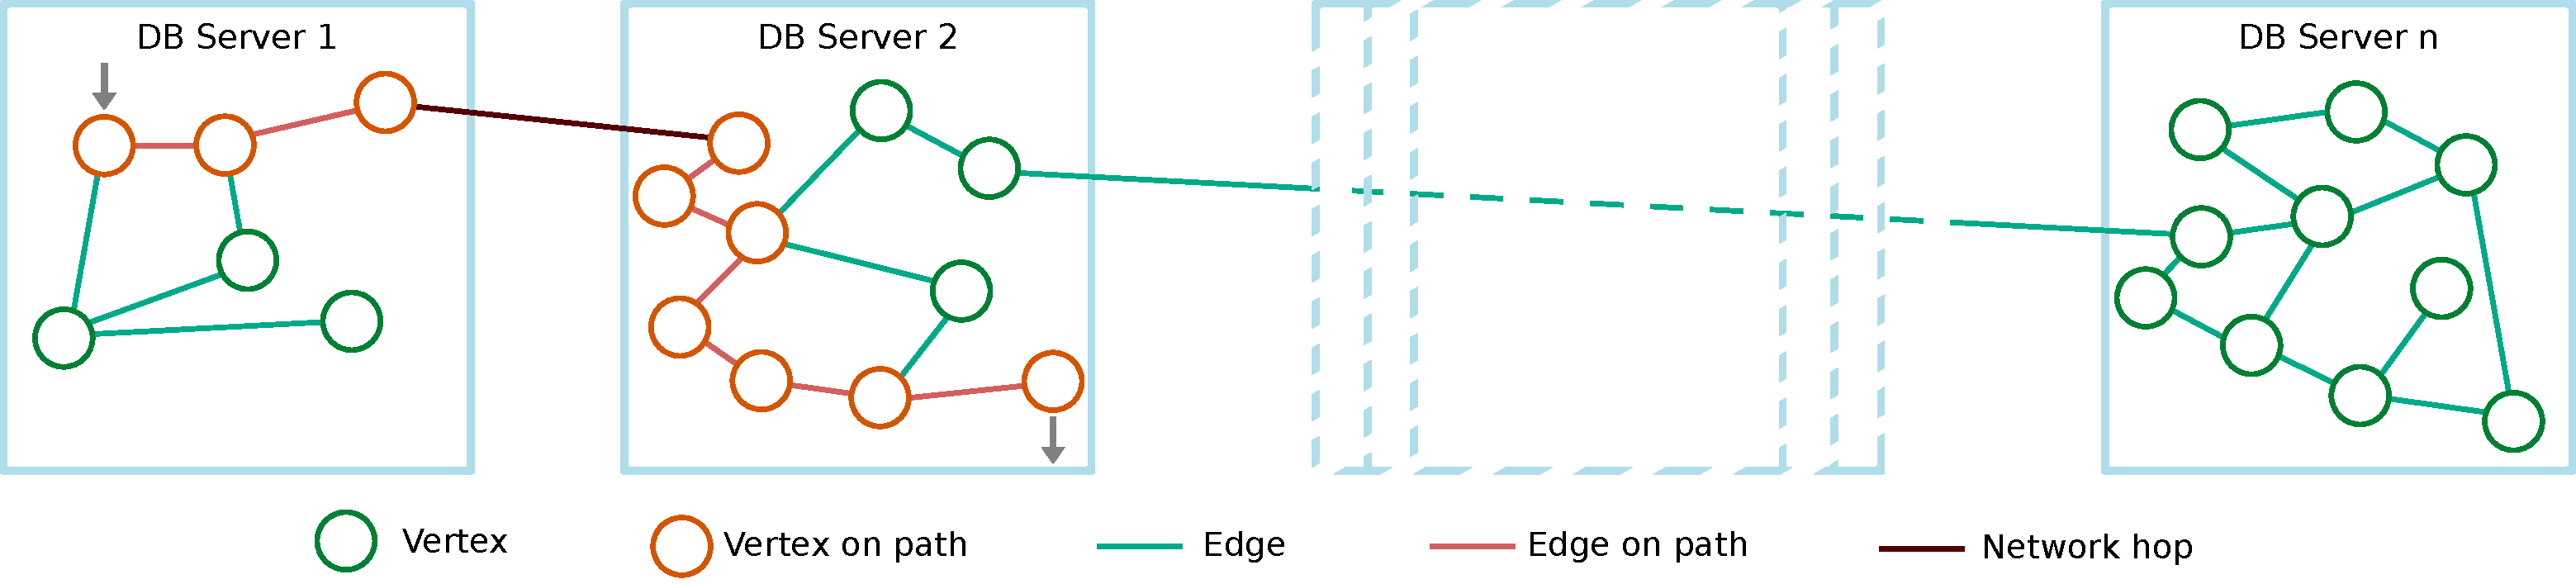
\includegraphics[width=1\textwidth,%
	]{images/chapter2/arangodbsmartgraphs.pdf}%
	\caption[ArangoDB's SmartGraphs for sharding]{ArangoDB's SmartGraphs for sharding}%
	\label{fig:arangodbsmartgraphs}%
\end{figure}%

ArangoDB may be horizontally scaled by using many servers.
Because of their nature, the data models created by ArangoDB offer different opportunities for scalability.
Particularly, the ability to scale decreases from key/value over documents (documents with joins) to graphs.
The key/value store data model is the most scalable since a document collection always has a primary key (\texttt{\_key} attribute) and document collections behave like simple key/value stores in absence of additional secondary indexes.
Single key lookups and key/value pair insertions and updates are the only logical in this situation.
If the key attribute is the only sharding attribute, sharding is done with respect to the primary key and all operations scale linearly.\sfcite{Sinico2017}
Even in presence of secondary indexes, the same is valid for the document store, because an index for a sharded collection is simply the same as a local index for each shard.
Each shard only stores the part of an index that it needs.
As a result, single document operations continue to scale linearly with cluster size.
However, because the \acrshort{AQL} query language permits queries to employ multiple collections, secondary indexes and joins, scalability might be difficult if the data to be combined is spread over numerous machines, as a lot of communication is required.
When working with graph data, the same thing happens.\sfcite{Sinico2017}

It is therefore, crucial to configure the graph data distribution across the shards in a well-studied manner in order to provide good performance at scale.
ArangoDB asks users to specify which attributes to utilize for the graph data to be sharded.
The suggestion is to make sure that edges originating at a node are located on the same cluster machine as the node itself.
ArangoDB Enterprise Edition, includes the SmartGraph feature, which implements graph partitioning based on community detection in order to reduce network communication.
The distributed architecture is managed by a multi-master model and a number of ArangoDB instances communicate with one another via the network and play different roles (Agents, Coordinators, Primary and Secondary DBservers).\sfcite{ArangoDBWhyArangoDB2021}

\subsubsection{Graph visualization}\label{subsubsection:LiteratureReview/ReviewofGraphDatabaseSystems/AGDBMSindetailArangoDB/Graphvisualization}
\begin{figure}[H]%
	\centering%
	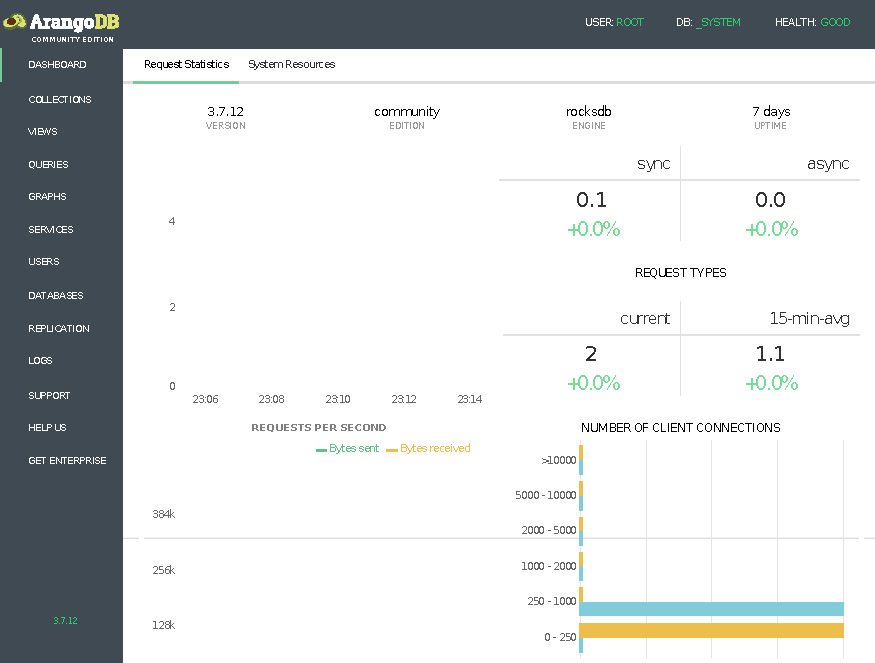
\includegraphics[width=1\textwidth]{images/chapter2/arangodbwebinterfacenew.pdf}%
	\caption[ArangoDB's Aardvark web interface]{ArangoDB's Aardvark web interface}%
	\label{fig:arangodbwebinterfacenew}%
\end{figure}%

ArangoDB comes with a useful web interface called Aardvark.
With this interface the database administrator can view some live statistics on the dashboard and perform operations like:
\setlist{nolistsep} \begin{itemize}[noitemsep]
	\item manage databases, collections and documents;
	\item execute and save \acrshort{AQL} queries;
	\item manage the database schema, impose constraints and create indexes;
	\item store and launch services/procedures;
	\item get a graph-representation of the data contained in the form of a graph model, as shown in \hyperref[fig:QueryResolverGraphBrugali]{\autoref{fig:QueryResolverGraphBrugali}} on \hyperref[fig:QueryResolverGraphBrugali]{page \pageref*{fig:QueryResolverGraphBrugali}};
	\item view the database logs.
	\item create, manage and explore graphs click-by-click;
	\item create new vertices and edges in an interactive way directly in the graph visualizer;
\end{itemize}

\subsubsection{Licensing}\label{subsubsection:LiteratureReview/ReviewofGraphDatabaseSystems/AGDBMSindetailArangoDB/Licensing}
ArangoDB offers three different levels of subscription\sfcite{ArangoDBSubscriptions2021, ArangoDBWhyArangoDB2021}:
\setlist{nolistsep} \begin{itemize}[noitemsep]
	\item The Community Edition is an open and free license without direct support and without custom advanced features.
		  It is released under the Apache v2 license.
		  Of all the major GDBMSs Community Editions, ArangoDB's CE is the one that provides the most features of its upgraded Enterprise Edition.
	\item The Enterprise Edition is a commercial license with dedicated support and contact to experts of the core team.
		  It includes all features of the Community version plus SmartJoins, SmartGraphs, Encryption, Auditing and training.
	\item The Oasis Edition offers fully managed service with physical or cloud machines.
\end{itemize}

With this ends the in-detail description of ArangoDB and this chapter altogether.
In the next one shall be presented the Label Propagation Community Detection algorithm and the usage of ArangoDB for the its application to cluster academic collaboration communities.

\newpage
\thispagestyle{empty}
